%\documentclass[draft]{ua-thesis}
\documentclass[final]{ua-thesis}
%<my packages>
%% Language and font encodings
\usepackage{gb4e}
\noautomath
\usepackage{natbib}
\usepackage[english]{babel}
\usepackage[utf8x]{inputenc}
\usepackage[T1]{fontenc}

%% Sets page size and margins
%\usepackage[a4paper,top=3cm,bottom=2cm,left=3cm,right=3cm,marginparwidth=1.75cm]{geometry}

%% Useful packages
\usepackage{amsmath}
\usepackage{graphicx}
\usepackage[colorinlistoftodos]{todonotes}
\usepackage[colorlinks=true, allcolors=blue]{hyperref}
\usepackage{fixltx2e}
\usepackage{rotating}
\usepackage{Sweave}

\newcommand*{\myfont}{\fontfamily{ccr}\selectfont}
%the newcommand change the selected word into 'ccr' font
%e.g. \begin{myfont} multi-bleu.perl \end{myfont}
%\<my packages>
%packages used by Koeh
\usepackage{url}
\usepackage{color}
\usepackage{epic,ecltree}
\usepackage{eclbip}
\usepackage{multicol}
\usepackage{algorithmic}
\usepackage{algorithm}
\renewcommand{\algorithmicrequire}{\textbf{Input:}}
\renewcommand{\algorithmicensure}{\textbf{Output:}}
\renewcommand{\algorithmiccomment}[1]{// {\em #1}}

\definecolor{darkblue}{rgb}{0,0,0.8}
\definecolor{darkgreen}{rgb}{0,0.8,0}
\definecolor{reddishgreen}{rgb}{0.4,0.6,0}
\definecolor{purple}{rgb}{0.6,0,0.6}
\definecolor{red}{rgb}{1,0,0}

\newcommand{\example}[1]{\textcolor{darkblue}{\rm #1}}
\newcommand{\maths}[1]{\textcolor{purple}{#1}}
\newcommand{\reference}[1]{\vspace{-2mm}\begin{flushright}\textcolor{purple}{\tiny [from #1]}\end{flushright}\vspace{-7mm}}
%End packages used by Koeh

\usepackage{verbatim}
%\usepackage{amssymb,amsmath,amsthm}
%\usepackage[mathscr]{eucal}

\usepackage{makeidx}
\numberwithin{equation}{section}
%\numberwithin{equation}{subsection}
%\input{isomath}
\input{mathenv}
\input{syms}
\usepackage{graphicx}
\usepackage{psfrag}
\usepackage{afterpage}
\usepackage{subfigure}
\usepackage{hyperref}
\usepackage{ifpdf}
\usepackage{qtree}
\usepackage{fixltx2e}
\graphicspath{ {figures/} }
\DeclareMathOperator*{\argmax}{argmax} 
\usepackage{tikz}
\usetikzlibrary{matrix,chains,positioning,decorations.pathreplacing,arrows}
\usetikzlibrary {positioning}




\director{Mike Hammond}


\author{Yuan-Lu Chen}
\title{Improving Neural Net Machine Translation Systems with Linguistic Information}
\date{2018}
\makeindex

\ifpdf
\pdfinfo{
/Author (Yuan-Lu Chen)
/Title  (Improving Neural Net Machine Translation Systems with Linguistic Information)
}
\fi

%% ================================================================
\begin{document}
\Sconcordance{concordance:RealMaster.tex:RealMaster.Rnw:%
1 79 1}
\Sconcordance{concordance:RealMaster.tex:./Introduction.Rnw:ofs 80:%
1 13 1}
\Sconcordance{concordance:RealMaster.tex:./gloss.Rnw:ofs 94:%
1 54 1}
\Sconcordance{concordance:RealMaster.tex:./Description_of_Corpus.Rnw:ofs 149:%
1 8 1}
\Sconcordance{concordance:RealMaster.tex:./intro_MT.Rnw:ofs 158:%
1 7 1}
\Sconcordance{concordance:RealMaster.tex:./RealCake.Rnw:ofs 166:%
1 154 1}
\Sconcordance{concordance:RealMaster.tex:./GLOSS_table.Rnw:ofs 321:%
1 1 17 23 0}
\Sconcordance{concordance:RealMaster.tex:./RealCake.Rnw:ofs 346:%
157 16 1}
\Sconcordance{concordance:RealMaster.tex:./RealCake2.Rnw:ofs 363:%
1 61 1}
\Sconcordance{concordance:RealMaster.tex:./ParaPart_table.Rnw:ofs 425:%
1 1 17 23 0}
\Sconcordance{concordance:RealMaster.tex:./RealCake2.Rnw:ofs 450:%
64 30 1}
\Sconcordance{concordance:RealMaster.tex:./Para_table.Rnw:ofs 481:%
1 1 17 23 0}
\Sconcordance{concordance:RealMaster.tex:./RealCake2.Rnw:ofs 506:%
96}
\Sconcordance{concordance:RealMaster.tex:./GDParaParaPart_null_table.Rnw:ofs 507:%
1}
\Sconcordance{concordance:RealMaster.tex:./RealCake2.Rnw:ofs 508:%
98 2 1}
\Sconcordance{concordance:RealMaster.tex:./GDParaParaPart_table.Rnw:ofs 511:%
1 1 19 23 0}
\Sconcordance{concordance:RealMaster.tex:./RealCake2.Rnw:ofs 536:%
102 18 1}
\Sconcordance{concordance:RealMaster.tex:./interleavingGdGLOSS_table.Rnw:ofs 555:%
1 1 17 23 0}
\Sconcordance{concordance:RealMaster.tex:./RealCake2.Rnw:ofs 580:%
122 21 1}
\Sconcordance{concordance:RealMaster.tex:./concat_table.Rnw:ofs 602:%
1 1 17 23 0}
\Sconcordance{concordance:RealMaster.tex:./RealCake2.Rnw:ofs 627:%
145 16 1}
\Sconcordance{concordance:RealMaster.tex:./ReplacingGaelic_table.Rnw:ofs 644:%
1 1 17 23 0}
\Sconcordance{concordance:RealMaster.tex:./RealCake2.Rnw:ofs 669:%
163 1 1}
\Sconcordance{concordance:RealMaster.tex:./ReplacingGLOSS_table.Rnw:ofs 671:%
1 1 17 23 0}
\Sconcordance{concordance:RealMaster.tex:./RealCake2.Rnw:ofs 696:%
166 5 1 1 11 23 0 1 2 18 1}
\Sconcordance{concordance:RealMaster.tex:./gloss_in_other_languages.Rnw:ofs 745:%
1 3 1}
\Sconcordance{concordance:RealMaster.tex:./Implications_ling.Rnw:ofs 749:%
1 1 1}
\Sconcordance{concordance:RealMaster.tex:./Conclusion.Rnw:ofs 751:%
1 1 1}
\Sconcordance{concordance:RealMaster.tex:RealMaster.Rnw:ofs 753:%
90 7 1}


\maketitle

\chapter*{Dedication}
\thispagestyle{topright}
\begin{center}For Eva, the best linguist in my world.\end{center}
\chapter*{Acknowledgments}
acknowledgment!
Many people help me and keep me company in my this journey.
Thank you.

\begin{vim_bug_workaround}
\end{vim_bug_workaround}


\tableofcontents
\listoffigures
\listoftables

\begin{abstract}
The gloss data that are widely used in theoretical linguistics are hidden treasures for machine translation. 
This dissertation introduces the gloss data to the natural language processing research field and demonstrates a practical and effective way to incorporate gloss data into the training data for training neural net machine translation systems. 
\end{abstract}

%\input{disbody.tex}

\printindex

\chapter{Introduction}
\label{chap:Introduction}

Key information to be included:
\begin{enumerate}
\item outline/organization of the dissertation 
\item Arguments to be made in the dissertation: 
	\begin{enumerate}
	\item To understand language, NLP and Linguistics should work together.
    \item  Gloss is the right `lingua franca' for the two fields.
    \item Linguistics helps NLP.
    \item NLP helps linguistics. 
	\end{enumerate}
\end{enumerate}
\chapter{What are glosses? Why are they golden representations of meanings?}
\label{chap:gloss}

\section{Introduction: What are Glosses?}

Interlinear Glossed Text is widely used in linguistic studies. The following is an example of Interlinear Glossed Text.
\begin{exe}  
\ex\label{gloss_eg} Indonesian \citep[p. 237]{sneddon2012indonesian}
	\gll   Mereka di Jakarta sekarang. (\textit{sentence of interest})\\
     	   they in Jakarta now (\textit{gloss line: word-by-word gloss translation})\\
    \glt   `The are in Jakarta now.' (\textit{English translation})  
\end{exe}

A chunk of an interlinear glossed text has three lines. The first line is the sentence of interest. The second line is the gloss line, which is a word-by-word translation of the first line. And the third line a free English translation of the first line.

The conventional way to show the word-by-word translation from the first line to the gloss line is to use vertical alignment. In (\ref{gloss_eg}), `\textit{Mereka}' is glossed as `\textit{they}', `\textit{di}' is glossed as `\textit{in}', `\textit{Jakarta}' is glossed as `\textit{Jakarta}', and `\textit{sekarang}' is glossed as `\textit{now}'. These pairs are vertically aligned. 

The gloss line also provides morphological information. Consider the following example:

\begin{exe}  
\ex French
	\gll   aux chevaux\\
     	   to.ART.PL horse.PL \\
    \glt   `to the horses'  
\end{exe}

The morphemes of a single word is linked by a `.'. The French word `aux' is actually a combination of three separate morphemes\footnote{A morpheme is a smallest unit of meaning. For example, `\textit{boys}' has two morphemes in it: `\textit{boy}' and `\textit{-s}', where `\textit{-s}' is a plural marker. Sometimes, the morpheme boundary is not visible. For example `\textit{went}' is composed of `\textit{go}' and `\textit{-ed}'.}: `\textit{to}', `\textit{ART}', and `\textit{PL}' and \textit{`chevaux'} is decomposed into \textit{`horse'} and \textit{`PL'}.   
\citet{bickel2008leipzig} compile a set of widely used conventions of IGT called the Leipzig Glossing Rules.
Note that they are just guidelines of the formats of Interlinear Glossed Texts, so that Interlinear Glossed Texts can be more standardized. 

The underlying intuition of Interlinear Glossed Text is that it provides an access to look into the subparts of a sentence. We may imagine the situation without the gloss line; then all we have is just the sentence and the English translation of that sentence. This will make it really hard to discuss the internal structure of the sentence. On the other hand, with the presence of the gloss line, with which each word is glossed and annotated, we then have a meta-representation in hand to discuss the grammatical properties of the sentence of interest.  
 
An important note of the gloss line is that it is NOT raw linguistic data, and it is already processed. A linguist has already committed to some theory or some analysis on the sentence of interest when he or she transcribes the sentence into a gloss line, even if he or she tries to be as neutral as possible. As such, the question of what the gloss of a word is not trivial at all. Actually, sometimes a whole linguistic paper or thesis is to discuss and argue what the right gloss for a word is.  

\begin{exe}  
\ex Mandarin Chinese
	\gll   Zhangsan \textbf{hen} gao\\
     	   Zhangsan HEN tall\\
    \glt   `Zhangsan is tall.'  
\end{exe}  

For example, \citet{grano2008mandarin}, \citet{Chen2010}, and \citet{liu2010positive} discuss the nature of the Mandarin Chinese word `\textit{hen}' in the above example and what the right gloss should be `\textit{hen}'. In cases like this, how one glosses a word is not trivial at all, but determining what the gloss of word is requires a set of evidence and arguments. 

\section{The Golden Properties of Glosses}

A system of meaning representations is decomposed of three components: a) meanings, b) representations, and c) a mapping between meanings and representations. The most ideal meaning representation system should be built with one-meaning-to-one-representation mappings; in other words, a meaning is mapped to one and only one representation. Natural languages fail to do so, given that synonyms and ambiguous words/phrases are ubiquitous in natural languages. On the other hand, gloss provides a mapping that is close to this ideal one-to-one mapping. Thus gloss should a better representation in term of representing meanings. 

Theoretically, the claim that gloss representation is closer to the ideal one-to-one mapping than natural language representation can be tested empirically. 
Let's imagine a set of special golden meta-linguistic semantic representations, which has the following property: each concept is mapped to one and only one representation and each representation is mapped to one and only one concept. With this imaginary golden semantic representation system, we may now compare Gaelic words and glosses. First, it is expected that each golden representation token will map to more natural language words than gloss items do.

\begin{exe}
\ex
	\begin{xlist}
	\ex \label{gold_to_gd} $golden_i \rightarrow \{Gaelic\_word_1, Gaelic\_word_2, \ldots\}_{golden_i}$
	\ex\label{gold_to_gl} $golden_i \rightarrow \{gloss_1, gloss_2, \ldots\}_{golden_i}$
	\ex\label{gd_gl_comp1}$ |\{Gaelic\_word_1, Gaelic\_word_2, \ldots\}_{gold_i}| \geq |\{gloss_1, gloss_2, \ldots\}_{gold_i}|$
	\end{xlist}
\end{exe}

(\ref{gold_to_gd}) and (\ref{gold_to_gl}) represent a singe golden token may maps to multiple Gaelic words and glosses respectively. If we compare the size of them, it is expected that the set of Gaelic words is bigger than that of glosses, meaning that Gaelic words are more likely to be homographs than glosses are. Section \ref{sec:cluster} will provide concrete examples to exemplify this property of glosses. 

For the other direction, we may determine which one, Gaelic words or glosses, is more likely to be ambiguous.   

\begin{exe}
\ex
	\begin{xlist}
	\ex \label{gd_to_gold} $Gaelic\_word_i \rightarrow \{golden_1, golden_2, \ldots\}_{Gaelic\_word_i}$
	\ex \label{gl_to_gold} $gloss_i \rightarrow \{golden_1, golden_2, \ldots\}_{gloss_i}$
	\ex\label{gd_gl_comp2}$ |\{golden_1, golden_2, \ldots\}_{Gaelic\_word_i}| \geq |\{golden_1, golden_2, \ldots\}_{gloss_i}|$
	\end{xlist}
\end{exe}

(\ref{gd_to_gold}) and (\ref{gl_to_gold}) show the mappings from a Gaelic word to different concepts and the mappings from a gloss to different concepts respectively. 
(\ref{gd_gl_comp2}) is the expectation that Gaelic words are more likely to be ambiguous than glosses are. Section \ref{sec:disa} will report concrete examples to show that glosses are less likely to be ambiguous.

To run statistical experiments to confirm the truth of (\ref{gd_gl_comp1}) and (\ref{gd_gl_comp2}) is the way to empirically support the claim that glosses closer to the golden representations than Gaelic words are. 
However, in reality, this is an impossible experiment to conduct, because there are no such golden representation\footnote{It would solve the puzzle of semantics if one should be able to build the set of special golden meta-linguistic semantic representations, and the mappings between the golden representations to natural languages.}.
In spite of the impossibility of conducting statistical experiments, we may still use some examples to show the intuition that glosses are better representations than natural languages are. The following sections describes how glosses cluster words with different forms but with the same meaning, and how glosses represent words with the same form but with different meanings with different representations. 

\subsection{Glosses Cluster Different Words with the Same Meanings (Synonyms) Into a Single representation}\label{sec:cluster}
Gloss collapses words with different forms with the same meanings into a single gloss. In natural languages, the morphology of a word (i.e. the form of a word) may be sensitive to the phonological environments and changing into different forms. Consider the following the indefinite article in the English examples: 

\begin{exe}  
\ex \gll John ate \textbf{an} apple.\\
	John eat.past	\textbf{INDF\_ART} apple\\
\ex \gll John ate \textbf{a} banana.\\
	John eat.past   \textbf{INDF\_ART} banana\\
\end{exe}

In the above example, \textit{an} and \textit{a} have the identical meaning\footnote{Semantically, \textit{an} and \textit{a} are existential quantifiers, which declare that a member of a set exists in the world. In formal semantics, \textit{an} and \textit{a} may be defined as follows: $\exists\lambda P[P(x)]$. In the current example, \textit{apple} and \textit{banana} will instantiate $P$ in the formula, and the meanings will be `an apple exists' and `a banana exists'. \citet{kratzer1998semantics} would be a nice introduction for interested readers to see how linguists, specifically semanticians, define, decompose, and compose meanings of languages formally.}. 
In English, the same concept is realized as two representations, \textit{a} or \textit{an}, while in the gloss representation the one concept is neatly represented as \textit{INDF\_ART} (indefinite article). 

Critically, synonyms like the English \textit{a} and \textit{an} commonly occur in many other natural languages if not in all languages. The definite article in the language of interest, Scottish Gaelic, is another example to show the noisiness of natural language representations. Consider the definite article in the following Gaelic examples. 

\begin{exe}  
\ex 
\gll tha mi a' sireadh \textbf{an} leabhair bhig ghuirm\\
be-PRES-IND 1S PROG searching-VN \textbf{ART} book-G small-G blue-G\\
\glt `I am looking for the small blue book' \citep[p. 29]{lamb2001scottish}

\ex 
\gll \textbf{am} fear m\`or\\
\textbf{ART} man big\\
\glt `a big man' \citep[p. 31]{lamb2001scottish}

\ex
\gll thuit \textbf{a'} chlach air cas mo mhn\`a\\
fall-PAST \textbf{ART} stone on foot 1S-POSS wife-G\\
\glt`the stone fell on my wife's foot' \citep[p. 30]{lamb2001scottish} 	

\ex
\gll doras \textbf{na} sgoile(adh) \\
door-N \textbf{ART} school-G \\
\glt `the door of the school' \citep[p. 29]{lamb2001scottish} 	

\ex 
\gll a chuir air d\`oigh \textbf{nan} \`airidhean a-muigh a rubh' Eubhal agus an oidhche seo \\
to put-INF on order \textbf{ART} sheilings out-LOC to point Eaval and ART night this \\
\glt `the girls big house' \citep[p. 100]{lamb2001scottish} 

\ex
\gll f\`eis \textbf{nam} b\`ard\\
festival \textbf{ART} poet.PL.GEN\\
\glt `festival of the poets' \citep[p. 107]{lamb2001scottish}

\end{exe}

The definite article in Scottish Gaelic may be realized as the following forms: \textit{an}, \textit{am}, \textit{a'}, \textit{na}, \textit{nan} or \textit{nam}. The alternation is determined by the case, gender and number of noun phrase that it modifies, and additionally the phonological property of the word following it also changes the form of the definite article \citep{lamb2001scottish}. All these different realizations refer to the same concept, the definite article. Again, the gloss notation nicely clusters them together as \textit{ART}. 

In Mandarin Chinese, similar patterns are found. Consider classifiers in the following examples:

\begin{exe}
\ex \label{chinese_cl_eg}
\gll Yani mai-le \{\textbf{pi}/\textbf{*tou}\} ma , Lulu mai-le \{\textbf{*pi}/\textbf{tou}\} zhu.\\ 
Yani buy-PRF CL/CL horse , Lulu buy-PRF CL/CL pig\\
\glt `Yani bought a horse and Lulu bought a pig.' \citep[p. 136]{zhang2013classifier}
\end{exe}

In \citet{zhang2013classifier}, the classifier like \textit{pi} and \textit{tou} is a type of \textit{indivual classifier} which co-occurs with countable nouns, like \textit{ma}, `horse', and \textit{zhu}, `pig', and this type of classifier is the head of \textit{UNIT Phrase}. 
\textit{Pi} and \textit{tou} actually have the same semantics and the syntactic function; however, they are realized in different forms, specifically the form of which has to agree with the noun following it (i.e. \textit{pi} goes with \textit{ma}; \textit{tou} goes with \textit{zhu}). Here the gloss, \textit{CL}, unifies the two forms of the same meaning.    

Gloss collapses synonyms in natural languages. Learning the general distribution of the article and all its different forms is a challenge for the MT system, but the glossing information should make this easier.

\subsection{Glosses Distinguish Homographs' Different Meanings}\label{sec:disa}

In natural languages, there are cases when a single form denotes distinct concepts. Words with this property are termed as homographs. Consider the word \textit{for} in following English examples:

\begin{exe}
\ex \label{for_eng}
	\begin{xlist}
	\ex \label{for_c}I intended \textbf{for} Jenny to be present.
	\ex \label{for_p}\textbf{For} Jenny, I intended to be present. \citep[p.306-307]{adger2003core}
	\end{xlist}
\end{exe}

\textit{For} in (\ref{for_c}) and (\ref{for_p}) has the same form but different meanings. Specifically, \textit{for} in (\ref{for_c}) is a complementizer with its part of speech being \textit{C}, and it heads the non-finite clause \textit{Jenn to be present}; on the other hand \textit{for} (\ref{for_p}) is a preposition, which takes a Determiner Phrase, \textit{Jenny}, as its benefactive argument.   

The Scottish Gaelic word \textit{a'} in the following examples also has different meanings.  

\begin{exe}  
\ex \label{a_prog}
\gll tha mi \textbf{a'} sireadh an leabhair bhig ghuirm.\\
be-PRES-IND 1S \textbf{PROG} searching-VN ART book-G small-G blue-G\\
\glt `I am looking for the small blue book.' \citep[p. 29]{lamb2001scottish}

\ex \label{a_det}
\gll thuit \textbf{a'} chlach air cas mo mhn\`a.\\
fall-PAST \textbf{ART} stone on foot 1S-POSS wife-G\\
\glt`the stone fell on my wife's foot.' \citep[p. 30]{lamb2001scottish} 	
\end{exe}

Critically \textit{a'} in (\ref{a_prog}) is a progressive aspect marker while the same form in (\ref{a_det}) is a definite article. Again, the semantic difference is preserved in the gloss representations but not in natural language words. As such, the usefulness of glosses becomes very apparent.  

\subsection{Glosses are Sensitive to Hierarchical Structures in Natural Language Sentences}

Before I introduce how gloss information is linked to hierarchical structures, it is necessary to emphasize the importance of hierarchical structures in natural languages. In this section, I will first review some linguistic arguments for why and how semantics and syntax of languages\footnote{When it turns to the sound aspect of languages, Phonetics is more about linear order, but Phonology is still sensitive to hierarchical structures just like syntax and semantics. } are all about hierarchical structures instead of linear word orders. Then I will link gloss to hierarchical structures.

It is well-argued in linguistics that the syntax and semantics of natural languages are determined by hierarchical structures instead of linear orders of words, and essentially it is the sensitivity of hierarchical structures that distinguishes human natural languages from other animal communications \citep{berwick2015only}.     

Semantics is determined by hierarchical structures instead of linear orders. \citet[p. 117]{berwick2015only} use the following simple example to demonstrate this property of natural languages:

\begin{exe}
\ex Instinctively birds that fly swim. 
\end{exe}

In the example above, \textit{instinctively} is linearly closer to \textit{fly} than \textit{swim}; however, it unambiguously modifies \textit{swim} instead of \textit{fly}. The reason for this is the hierarchical structures \citep[p. 117]{berwick2015only}:

\begin{exe}
\ex \label{tree}
\Tree [Instinctively [ [  birds   [  that   fly  ]  ]  swim  ] ]
\end{exe}

In (\ref{tree}) it is shown that \textit{fly} is more embedded than \textit{swim}, and thus it is hierarchically further away from \textit{instinctively}. So, \textit{instinctively} can only modify \textit{swim} instead of \textit{fly}.

Syntax is also all about hierarchical structures. Consider the following sentence:

\begin{exe}
\ex 
	\begin{xlist}
	\ex \label{aux_inver1} Birds that can\textsubscript{1} fly can\textsubscript{2} swim. 
	\ex \label{aux_inver2} *Can\textsubscript{1} birds that  fly can\textsubscript{2} swim? 
	\ex \label{aux_inver3} Can\textsubscript{2} birds that can\textsubscript{1} fly  swim? 
	\end{xlist}
\end{exe}

(\ref{aux_inver1}) is a declarative sentence. To derive an interrogative sentence from it, the auxiliary needs to be moved; however, only \textit{can\textsubscript{2}} can be moved but not \textit{can\textsubscript{1}}, even thought \textit{can\textsubscript{1}} is linearly closer to the sentence initial position. Again, it is all because of the hierarchical structures. \textit{Can\textsubscript{2}} is in the matrix clause while \textit{can\textsubscript{1}} is in the embedded relative clause.

%Word order and linearizion are just epiphenomena from the perspective of theoretical syntax and semantics. They are inevitable externalizations of language because we are living in a world of linear time and space. 
%To put this argument in another way, if externalization should be the primary nature of language, we should expect that some natural human languages should have manipulated the linear order of words in a sentence to express different meanings, because linear order is the externalization of language. However, this is not the case. No language exploits linear order, and instead universally language uses hierarchical structures, which is more difficult to be externalized than linear order. \citet{chomsky2006language} uses the following examples to illustrate this point.

% \begin{exe}
% \ex
% 	\begin{xlist}
% 	\ex\label{c1} Smart eagles can swim.
% 	\ex\label{c2} *Eagles smart can swim?
% 	\ex\label{c3} Can smart eagles swim?
% 	\end{xlist}
% \end{exe}

% (\ref{c1}) is a declarative sentence. (\ref{c2}) tries to swap the first two words to derive an interrogative sentence, and fails. (\ref{c3}) is the real interrogative sentence in natural languages. If externalization are the primary nature of language, it is expected (\ref{c2}) to be a common pattern in languages, because (\ref{c2}) exploits linear order, which is the externalization of language and the linear order serves the communication purpose just fine given that humans' cognition system is able to tell the difference between (\ref{c1}) and (\ref{c2}). 
%However, the pattern in (\ref{c2}) is not found in any human language; instead, (\ref{c3}) is used, which uses hierarchical structure relations. In term of externalization, (\ref{c2}) is more economical than (\ref{c3}) given that (\ref{c2}) only moves two positions of words while (\ref{c3}) moves three positions of words. Again, if externalization are the primary nature of language, language should have evolved the pattern of (\ref{c2}). Based on the fact that no language exploits linear order, it is argued that language externalization in particular are accessory.}.   

Glosses, on the other hand, are sensitive to the internal hierarchical structures or constituency of sentences. They provide more clues of the internal hierarchical structures or constituency of sentences than natural language words. Consider the following examples, modified from (\ref{for_eng}):

\begin{exe}
\ex
For as \textit{complementizer} (glossed as \textit{complementizer})
	\begin{xlist}
	\ex I intended \textbf{for} [Jenny] to be present.
	\ex I intended \textbf{for} [the girl] to be present.
	\ex I intended \textbf{for} [the little girl] to be present.
	\ex I intended \textbf{for} [the little girl who wants to eat some ice scream] to be present. 
	\end{xlist}
\ex
For as \textit{preposition} (glossed as \textit{preposition})
	\begin{xlist}
	\ex \textbf{For} [Jenny], I intended to be present. 
	\ex \textbf{For} [the girl], I intended to be present. 
	\ex \textbf{For} [the little girl], I intended to be present. 
	\ex \textbf{For} [the little girl who wants to eat some ice scream], I intended to be present. 
	\end{xlist}
\end{exe}

Linear length of the argument of \textit{for} (i.e. the sequences in the square brackets) does not have any effect in determining what the gloss is, and instead it is the hierarchical structures that determines what the gloss is. Then the form of gloss hints to the internal structures of the sentence. 

A even more dramatic example comes from Mandarin Chinese. A single sequences of words may have distinctive meanings because of different parses, and the difference of parses is marked by the differences of glosses. In the following examples, the sentence `\textit{Lao3Li3 mai3 hao3 jiu3}'\footnote{These specific examples are extensively discussed in Mandarin Chinese Tone Sandhi literature (e.g. \citet{cheng1973synchronic, mei1991tone, shih1997mandarin, wang2011variation}). Critically, the constituency plays a role in Mandarin Chinese Tone Sandhi.} may have two distinct meanings depending on the status of `\textit{hao3}'.    

\begin{exe}
\ex\label{hao1}
	\begin{xlist}  
		\ex 
		\gll   Lao3Li3 mai3 hao3 jiu3\\
     	   Laoli buy \textbf{Perf} wine \\
   		\glt   `Laoli bought a wine'
   		\ex \Tree [ Laoli [ [ buy \textbf{perf} ] wine ] ]
	\end{xlist}    
\end{exe}

\begin{exe}
\ex\label{hao2}
	\begin{xlist}  
		\ex 
		\gll   Lao3Li3 mai3 hao3 jiu3\\
     	   Laoli buy \textbf{good} wine \\
   		\glt   `Laoli buys a good wine'
   		\ex \Tree [ Laoli [ buy [ \textbf{good} wine ] ] ]
	\end{xlist}    
\end{exe}

In sentence (\ref{hao1}), `\textit{hao3}' goes with the verb `\textit{mai3}'; as such `\textit{hao3}' is interpreted as a Perfective marker and glossed as `\textit{Perf}'; on the other hand, in (\ref{hao2}), `\textit{hao3}' goes with the noun `\textit{jiu3}' and works as an adjective modifying `\textit{jiu3}', and it is glossed as `\textit{good}'. 

With all the examples above, we have showed that gloss lines provide more clues of the the internal structures of the sentences are than natural language words do. 

In the machine translation literature, it has been shown that the information of syntax and sentence parses can improve the quality of machine translation \citep{Syntax_to_Translation} and increase the accuracy of extracting thematic role relations in a sentence \citep{Semantic_Role_Labeling}. Given that glosses encode some sentence parse information, it is reasonable to hypothesize that glosses will improve machine translation.      

\section{Conclusion: What Is a Gloss Line and Why Do They Matter?} 
The gloss line is like a linguistic version of `word embedding'. A natural language word is first converted to a gloss, which is readable for linguists. 
Also we may view a gloss line as an artificial sentence using the purified `gloss words', a meaning representation with which one meaning is mapped to one and only one representation. It is a useful and widely used annotation algorithm that requires linguistic knowledge. Given the properties of gloss data, it can be a very useful data for machine translation. Moreover, gloss data is widely used in linguistics literature, so data is already out there and all we need to do to clean the data.
A loose end here is that, even if all the arguments should be sound, we still have no statistical evidence to show the usefulness of the gloss data. Chapter \ref{chap:cake} and \ref{chap:cake2} tie up this loose end, in which I will report machine translation experiments using gloss data.  
%\SweaveInput{Description_of_Corpus.Rnw}
\chapter{A General Introduction of Machine Learning and Machine Translation}
\label{chap:MT}

	\begin{enumerate}
	\item General review of supervised Machine learning \citep{kotsiantis2007supervised}: The goal is provide a high level of understanding of what machine learning is. Machine Learning is to learn from EXAMPLES/SAMPLES. For example, to define the meaning of `dog', instead of giving all the definable features of `dog', we feed the machine with as many as possible of information of entities of dogs that we have access. Montague Semantics is actually a variant of ML, within which `dog' is defined as `the set of all the dog that exists in the current world.'. As such, Montague Semantics is Machine Learning, because instead of defining 'dog' with certain arbitrary rules (+/- FEATURE), it says 'all the dogs entities in the current world'. Definition by samples/examples not by rules.    
	\item Literature on machine translation: from statistical machine translation \citep{koehn2009statistical} to neural machine translation \citep{cho2014learning,cho2014properties,bahdanau2014neural, Koehn_NMT2017}. (Target audience: linguists)
	\end{enumerate}

The current Chapter provides a general literature review and introduction of Machine Learning and Machine Translation, before I report neural net machine translation experiments in Chapter \ref{chap:cake}, \ref{chap:cake2} and \ref{chap:Tying_Up}. The purpose of current Chapter is not meant to be a comprehensive summary of all the technical details of Machine Learning and Machine Translation, but instead this chapter aims to provide high-level descriptions of the algorithms used in Machine Learning and Machine Translation. 

\section{What is Machine Learning?}

This section provides a general, brief and non-technical introduction of Machine Learning.

\subsection{What is a Function and What is a Model?}
Machine learning is a specific algorithm that builds a function. Before we touch upon machine learning, we need to talk about what a function is. Here a function simply means a mapping from an object to another object; to put it in another way, a function takes an input and returns an output. A general form of function is given below:

\begin{exe}
\ex $f: X \rightarrow Y$\\
	or \\
	$ y=f(x) $
\end{exe} 


For example, the following is a simple function that takes a number as input and returns the double of that number:

\begin{exe}
\ex \label{math_function}
\begin{xlist}
\ex $f(x)=2x$
\ex $f: x \rightarrow 2x $\\
	e.g.
	\begin{xlist}
	\ex $f: 1 \rightarrow 2$
	\ex $f: 2 \rightarrow 4$
	\ex $f: 3 \rightarrow 6$
	\ex $\dots$
	\end{xlist}
\end{xlist}
\end{exe}

Grammaticality judgment of a sequence of strings can be viewed as a function, where the input is the sequence and the output is either grammatical or ungrammatical.  

\begin{exe}
\ex 
\begin{xlist}
\ex $English\ Grammar: String \rightarrow Grammaticality$\\
	e.g.
	\begin{xlist}
	\ex $English\ Grammar:  John\ loves\ Mary \rightarrow grammatical $
	\ex $English\ Grammar: loves\ John\ Mary \rightarrow ungrammatical $
	\ex $\dots$
	\end{xlist}
\end{xlist}
\end{exe}

Translation can be viewed as function, too, where the input is a sentence in the source language and the output is a sentence in the target language that conveys the same meaning of the source sentence. For example, a function that translates Scottish Gaelic into English looks like:   

\begin{exe}
\ex 
\begin{xlist}
\ex $Translation_{GaelicToEnglish}: Gaelic\ sentence
 \rightarrow English\ sentence$\\
	e.g.
	\begin{xlist}
	\ex $Translation_{GaelicToEnglish}:\\
	  thuit\ a'\ chlach\ air\ cas\ mo\ mhn`a\\ 
	  \rightarrow\\
	   the\ stone\ fell\ on\ my\ wife's\ foot $
	\ex $Translation_{GaelicToEnglish}:\\
	  tha\ mi\ a'\ sireadh\ an\ leabhair\ bhig\ ghuirm\\
	  \rightarrow\\
	   I\ am\ looking\ for\ the\ small\ blue\ book $
	\ex $\dots$
	\end{xlist}
\end{xlist}
\end{exe}

Expect for mathematical functions like (\ref{math_function}), in most of the cases, we have no direct access to a function. In other words, the function is assumed to be unknown. 
To simulate the behaviors of an unknown function, we build a model with the hope that the model can do the same mapping as the target function.     
Schematically, the relation between a function and a model that simulates that function is depicted below:

\begin{exe}
\ex 
	\begin{xlist}
	\ex \label{fun_dipc} $f: X \rightarrow Y$ (unknown target function)
	\ex \label{model_dipc}$g: X \rightarrow \hat{Y}$ (model)\\
	where $Y \approx \hat{Y}$ 
	\end{xlist}
\end{exe}

(\ref{fun_dipc}) is the unknown target function (conventionally it is represented by $f$ in the literature), and (\ref{model_dipc}) is the model that we build with the hope that it does the same mapping as $f$ (conventionally a model is represented by $g$ in the literature).

In a nutshell, a model is a set of handmade mappings that simulates an unknown function. 

\subsection{Two Different Paradigms of Building a Model}

Now the critical problem is how we build a models to approximate the golden target function. With the unknown target function being the same $f$, there can be two distinctive approaches of building the model: Human-Reasoning Approach and Machine-Learning Approach. 

\begin{exe}
\ex Human-Reasoning Model:
A set of rules manually written by a human that attempts to approximate $f$ based on his or her own knowledge and experiences. 
\end{exe}

The Human-Reasoning approach is built on an individual's knowledge and is task-specific. 
Taking the English grammaticality judgment task as example, this approach will mean that some expert in English grammar will come up a set of rules or some algorithms that can determine whether a sequence of strings is a grammatical English sentences. 
The rules and algorithms are based on this expert's knowledge and they are English specific, and are not applicable to other language.     


Another approach to build a model is using Machine Learning. Instead of building a model from our own reasoning, we may look and all the available examples and come up with a generalization. This is the Machine Learning approach. 
Machine Learning can be defined as follows:

\begin{exe}
\ex Definitions of Machine Learning:
\begin{xlist}
	\ex Machine learning is based on algorithms that can learn from data without relying on rules-based programming \citep{pyle2015executive}. 
	\ex Machine learning algorithms can figure out how to perform important tasks by generalizing from examples \citep{domingos2012few}.
	\ex The field of Machine Learning seeks to answer the question `How can we build computer systems that automatically improve with experience, and what are the fundamental laws that govern all learning processes?' \citep{mitchell2006discipline}.
\end{xlist}
\end{exe}   

For the Machine Learning approach, the most critical factors of how a model is built are 1.) the generic learning algorithms and 2.) the input data from which the generic learning algorithms learns to set up the parameters of the derived model.  

Taking the English grammaticality judgment task as example again, the machine learning approach will first define some generic learning algorithms and then feed the algorithms with labeled sequences, where the label is either `grammatical English sentence' or `ungrammatical English sentence'. Note that the learning algorithms is generic. This means that it is universally applicable. For example, instead of feeding the learning algorithms with English grammaticality label, we may feed the learning algorithms with Scottish Gaelic grammaticality label, and it will able to derive a model that can tell whether a sequence of strings is a grammatical Scottish Gaelic sentence. 


In the genericness and universality of the learning algorithms, there is a reminiscence of Universal Grammar \citep{chomsky2007}. 
Universal Grammar is a type of machine learning. Instead of teaching a set of rules, the children is giving a set of grammatical sentences and then they are able to learn grammar, and produce grammatical sentences. 

\citet{chom2005_three_factors} describes three factors in language design: 1) Universal Grammar, 2) Experience, and 3) other cognitive mechanisms/limitations. This is actually a precise description of how machine learning works. Universal Grammar is the generic learning algorithm. Experience is the training data. Cognitive mechanisms are all the other hardware specification of a machine (i.e. a human brain). So, when the Experience is language X, a child acquires language X.  

  

%\section{A Overview of Theories in Machine Translation}

\section{Statistical Machine Translation}
Statistical Machine Translation uses statistical Machine Learning approaches to build machine translation systems \citep{brown1988statistical, brown1990statistical, brown1993mathematics, koehn2009statistical, moses}. The goal is to build a model that simulates the unknown language mapping function. The training data is parallel corpus, which a collection of pairs of a sentence in one language and the translation of the sentence in another language.

The fundamental translation equation of Statistical Machine Translation is shown as follows:

\begin{equation}
Pr(T|S)=\frac{Pr(T)Pr(S|T)}{Pr(S)}
\end{equation}

In this equation, we try to translate a sentence $S$ in the source language to a sentence $T$ in the target language. The left part of the equation represents the probability of $T$ given $S$. 
The right side of of the equation just flips the conditional probability using Bayes' theorem. 
The advantage of the flipping is that now $Pr(T)$ (the probability of sentence $T$). 
This information can be retrieved by building a language model of the target language, which can estimate the probability of a sequence of strings. $Pr(S|T)$ is the translation model, which measures the probability of $S$ given $T$. 
Given this equation, translating a given sentence $S$ simply means to find a sentence $\hat{T}$ that maximize $Pr(T|S)$.   

\begin{equation}
\hat{T}= \argmax_{T} Pr(T|S) = \argmax_{T} \frac{Pr(T)Pr(S|T)}{Pr(S)} = \argmax_{T} Pr(T)Pr(S|T)
\end{equation}

Now a Statistical Machine Translation system is decomposed into two sub-models: the language model of the target and the translation model. 
To build the language model, the common practice is to train a N-gram model given a corpus. 
To build the translation model, we will need to use parallel corpus. 
To understand the nature of Statistical Machine Translation, we need to look into what information is extracted from the parallel corpus. Critically, the probability of words in the source language aligned with words in the target language is the center of the translation model of Statistical Machine Translation. 

Given how Statistical Machine Translation builds the translation model, Statistical Machine Translation may be viewed as a complicated algorithm of string manipulations and string alignments. 
Importantly, this means that Statistical Machine Translation does not touch upon meaning, which limits the development and performance of Statistical Machine Translation. 

As such, Statistical Machine Translation is doomed to be outperformed by other deeper algorithms that touch upon the domains of meaning. Specifically, 2016 is the year when neural net machine translation started to outperform Statistical Machine Translation. In the Conference on Machine Translation 2016, a neural machine translation system outperformed almost every statistical machine translation systems. And in the following year, the Conference on Machine Translation 2017 went neural. Almost all the submitted papers and models were using neural net machine translation systems. 

In the next section, I will introduce the basics of artificial neural nets and the overview of how neural net machine translation.  

\section{Neural Net Machine Translation}\label{neural_MT}

\subsection{What Is a Artificial Neural Network?}

An artificial neural network is a simple but powerful computation algorithm. It can be viewed as a mathematical function: given an number or a vector of numbers as the input, it will return one and only number or vector. 

Historically, the basic structure of artificial neural networks was long completed more than 60 years ago, 
as \citet{rosenblatt} described the design and structure of a perceptron, which is the simplest artificial neural networks. 

\begin{figure}[h]
\caption{An Example of a Perceptron}
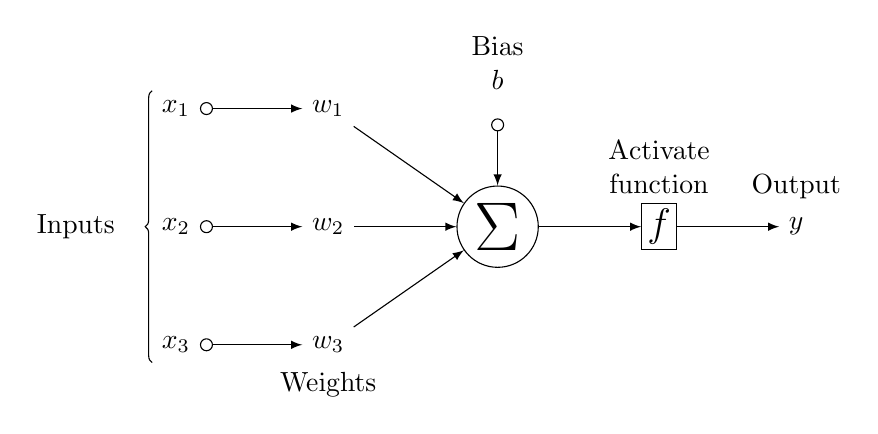
\begin{tikzpicture}[
init/.style={
  draw,
  circle,
  inner sep=2pt,
  font=\Huge,
  join = by -latex
},
squa/.style={
  draw,
  inner sep=2pt,
  font=\Large,
  join = by -latex
},
start chain=2,node distance=13mm
]
\node[on chain=2] 
  (x2) {$x_2$};
\node[on chain=2,join=by o-latex] 
  {$w_2$};
\node[on chain=2,init] (sigma) 
  {$\displaystyle\Sigma$};
\node[on chain=2,squa,label=above:{\parbox{2cm}{\centering Activate \\ function}}]   
  {$f$};
\node[on chain=2,label=above:Output,join=by -latex] 
  {$y$};
\begin{scope}[start chain=1]
\node[on chain=1] at (0,1.5cm) 
  (x1) {$x_1$};
\node[on chain=1,join=by o-latex] 
  (w1) {$w_1$};
\end{scope}
\begin{scope}[start chain=3]
\node[on chain=3] at (0,-1.5cm) 
  (x3) {$x_3$};
\node[on chain=3,label=below:Weights,join=by o-latex] 
  (w3) {$w_3$};
\end{scope}
\node[label=above:\parbox{2cm}{\centering Bias \\ $b$}] at (sigma|-w1) (b) {};

\draw[-latex] (w1) -- (sigma);
\draw[-latex] (w3) -- (sigma);
\draw[o-latex] (b) -- (sigma);

\draw[decorate,decoration={brace,mirror}] (x1.north west) -- node[left=10pt] {Inputs} (x3.south west);
\end{tikzpicture}
\end{figure}

In a perceptron, we have input nodes, which carry numerical values. These input nodes are connected to another node via weighted connection arrows. The newly linked node will have first has a raw numerical value. This raw value is simply the summation of the product of the numerical value of the input node and the weight of the linking arrow plus the bias value. In the example above, we will have:

\begin{exe}
\ex Raw numerical value= $x_{1}w_{1}+x_{2}w_{2}+x_{3}w_{3}+b$
\end{exe}

Then an activation function will further normalize the raw numerical value by mapping it to another value. 

\begin{exe}
\ex $y=f(Raw\ numerical\ value)$
\end{exe}

The most commonly used activation functions in artificial neural nets are Hyperbolic tangent, Logistic, and ReLU.

Here $y$ is the final output,which is another numerical value. A perceptron is the central building blocks of neural network computation. 

\begin{figure}
\caption{Activation functions}
\centering
\includegraphics[width=0.9\textwidth]{activation_function.png}
\end{figure} 

Note that the output of a perceptron can the the input of another perceptron. 
In this manner, the perceptron can interconnected to one and other yielding complicated networks. 

\begin{figure}[h]
\caption{A neural network with a hidden layer}
\centering
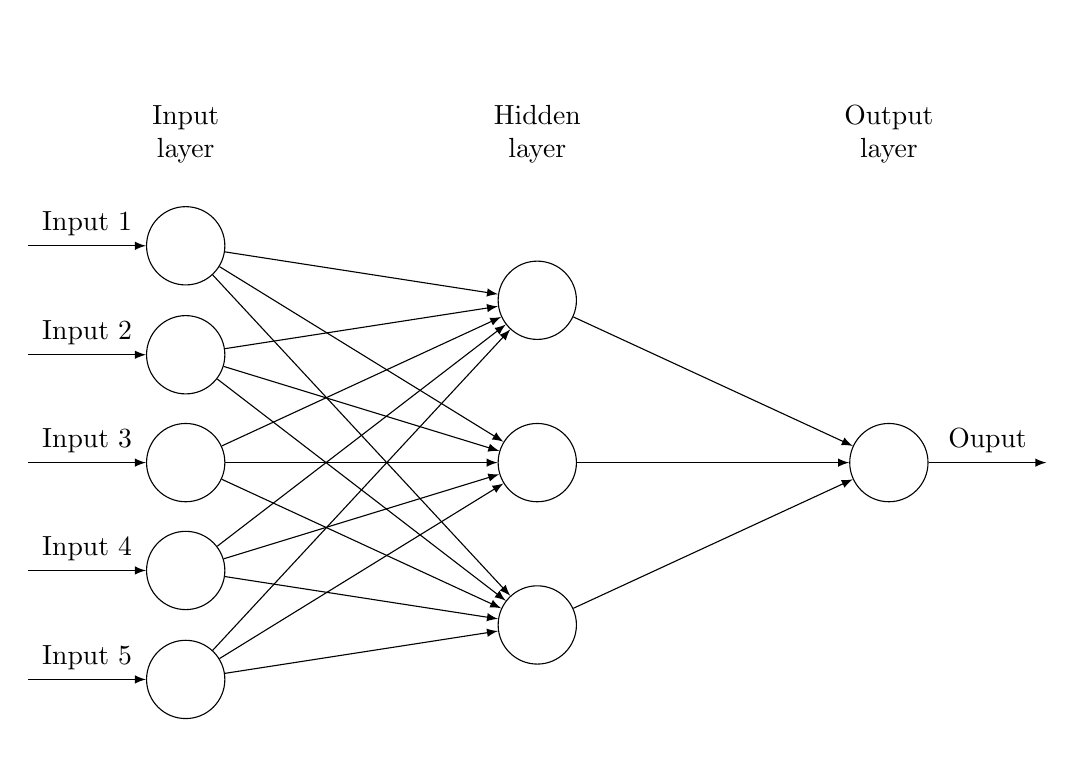
\begin{tikzpicture}[
plain/.style={
  draw=none,
  fill=none,
  },
net/.style={
  matrix of nodes,
  nodes={
    draw,
    circle,
    inner sep=10pt
    },
  nodes in empty cells,
  column sep=2cm,
  row sep=-9pt
  },
>=latex
]
\matrix[net] (mat)
{
|[plain]| \parbox{1.3cm}{\centering Input\\layer} & |[plain]| \parbox{1.3cm}{\centering Hidden\\layer} & |[plain]| \parbox{1.3cm}{\centering Output\\layer} \\
& |[plain]| \\
|[plain]| & \\
& |[plain]| \\
  |[plain]| & |[plain]| \\
& & \\
  |[plain]| & |[plain]| \\
& |[plain]| \\
  |[plain]| & \\
& |[plain]| \\    };
\foreach \ai [count=\mi ]in {2,4,...,10}
  \draw[<-] (mat-\ai-1) -- node[above] {Input \mi} +(-2cm,0);
\foreach \ai in {2,4,...,10}
{\foreach \aii in {3,6,9}
  \draw[->] (mat-\ai-1) -- (mat-\aii-2);
}
\foreach \ai in {3,6,9}
  \draw[->] (mat-\ai-2) -- (mat-6-3);
\draw[->] (mat-6-3) -- node[above] {Ouput} +(2cm,0);
\end{tikzpicture}
\end{figure}    


The following figure depicts a neural net with a hidden layer in the middle between the input and output nodes. When there are more than one hidden layer, the neural net is called deep neural net. However, the building blocks are still a simple perceptron. So, actually neural networks are simple and elegant computation operation\footnote{It seems to me that linking the perceptron is just like the simple Merge operation in the Minimalist Program.}; 
however, they extremely powerful. They are Turing-Complete machines \citep{siegelmann1991turing, graves2014neural}. \citet{siegelmann2003neural, siegelmann2012neural} even argues that neural networks are computations beyond the Turing limit. 

\subsection{Recurrent Neural Network}




\section{Introduction to Neural Net Machine Translation}

\begin{figure}[h]
\caption{Encoder-decoder architecture - example of a general approach for NMT. An encoder converts a source sentence into a "meaning" vector which is passed through a decoder to produce a translation. \citep{luong17GitHub}}
\centering
\includegraphics[width=0.9\textwidth]{encdec.jpg}
\end{figure} 


\begin{figure}[h]
\caption{Neural machine translation - example of a deep recurrent architecture proposed by for translating a source sentence ``I am a student'' into a target sentence ``Je suis \'{e}tudiant''. Here, ``<s>'' marks the start of the decoding process while ``</s>'' tells the decoder to stop. \citep{luong17GitHub}}
\centering
\includegraphics[width=0.9\textwidth]{seq2seq.jpg}
\end{figure} 

\begin{figure}[h]
\caption{Attention mechanism - example of an attention-based NMT system as described in \citet{luong2015effective}. Figure \citep{luong17GitHub}.}
\centering
\includegraphics[width=0.9\textwidth]{attention_mechanism.jpg}
\end{figure} 



\section{A Quick Historical Overview of Machine Translation and Conclusion}

Machine Translation is to automate the process of translating one natural language to another with using computers. The first peak of the developments of Machine Translation started in the 1940s but terminated in 1966. During this period of time, with the advent of the first computers, researchers held high expectations in Machine Translation and lots of resources are shifted into this area. However, in 1966 a report of the Automatic Language Processing Advisory Committee \citep{pierce1966language} terminated this `machine translation rush' as it revealed that too many funds and resources were shifted to Machine Translation without yielding proportional scientific developments. In 1990s, with the advent of Statistical Machine Translation approach developed at IBM, the Machine Translation came back as one of popular scientific areas. Now with the advent of the technique of Artificial Neural Net Machine Learning and other natural language process, Machine Translation is one of the most dynamic research areas.    
\chapter{Building Translation Systems using Interlinear Glossed Text: First Attempt}
\label{chap:cake}


\section{Introduction}
The Innovation is to incorporate the gloss information of Interlinear Glossed Text data into machine translation.

In supervised machine learning models, two factors effects the performance of the trained systems \citep{kotsiantis2007supervised}: a.) the quality of the training data and b.) the choice of the features. The properties of the gloss data as described in chapter \ref{chap:gloss} make it a better training data than natural language data (Scottish Gaelic in the current case) for the following reasons. First, glosses are more purified than natural language words. The most ideal meaning representation system should be built with one-meaning-to-one-representation mappings; in other words, a meaning is mapped to one and only one representation. Natural languages fail to do so, given that synonyms and ambiguous words/phrases are ubiquitous in natural languages. Glosses provide this one-to-one mapping. Second, the gloss data provides hierarchical (non-linear) syntactic parsing information. To determine what the gloss of a word is, linguists have to look for hierarchical (non-linear) context information. See chapter \ref{chap:gloss} for the discussion on the golden properties of glosses.  

Therefore, theoretically incorporation of the gloss data should improve the translation systems. Specifically, I propose the following hypothesis:
\begin{exe} 
\ex \label{gloss_helps_hypothesis}\textbf{Gloss-helps hypothesis: the translation systems trained with the gloss data incorporated should outperform the systems trained with only Gaelic and English sentences pairs (i.e. without gloss data).}

The hypothesis can have two versions, strong and weak:
	\begin{xlist}
	\ex \label{strong_hy} Strong version: Gloss may replace the source natural language totally, and the system outperforms the system trained with source natural language to target language sentence pairs (i.e. the baseline systems).  
	\ex \label{weak_hy} Weak version: Gloss only increases the performance of the baseline systems, but cannot replace the source language.
	\end{xlist}
\end{exe}

The experiments in the current chapter will reveal that replacing Gaelic words with glosses doesn't boost up the performance of the translation systems. Thus, the strong version (replacing-Gaelic-with gloss) of the Gloss-helps hypothesis is not empirically supported. 

This chapter describes the experiments conducted to test the strong version of the Gloss-helps hypothesis.
The rest of the chapter is organized as follows: Section \ref{relate_work} describes related works in the literature, Section \ref{sec:experimet_setting} describes the constant parameter settings across all the experiments and the corpus used in the experiments, Section \ref{gd_to_gl_to_en} tests the hypothesis in (\ref{strong_hy}), Section \ref{section:cake1_Discussion} discusses the results and conclude this chapter.
%%%%%%%%%%%%%%%%%%%%%%%%%%%%%%%%%%%%%%%%%%%%%%%%%%%%%%%%%%%%%%%%%%%%%%%%%%%%%%%%%%%%%%%%%
\section{Related Work}\label{relate_work}
Attempts to improve machine translation systems by incorporating explicit linguistic information are reported in the literature. Syntax information is known to be effective in improving statistical machine translation (SMT). The efforts of using syntax information even derive a special type of SMT, termed as syntax-based SMT \citep{williams2016syntax}. The same trend is also found in neural net machine translation. For example, \citet{sennrich2016linguistic} exploit the information of lemmas, part of speech tags, morphology of words, and dependency parses of sentences to improve MT systems. \citet{ccg_target_seq} incorporate the Categorial grammar parse tags of the target sequences.

%%%%%%%%%%%%%%%%%%%%%%%%%%%%%%%%%%%%%5

\section{Technical Settings of the Machine Translation Experiments and Experimental Data of Scottish Gaelic Interlinear Glossed Text Corpus}\label{sec:experimet_setting}

\subsection{Technical Settings}
The experiments are conducted by using OpenNMT \citep{2017opennmt}, which implements the state-of-the-art neural net machine translation algorithms \citep{cho2014properties, cho2014learning, bahdanau2014neural}.
The following default hyper-parameter settings of OpenNMT\footnote{See their documentation for the complete default hyper-parameter settings: \url{http://opennmt.net/OpenNMT-py/}.} are used across all models so that the only independent variable is the type of the training data:
	\begin{itemize}
	\item Word vector size: 500\\
	In neural net machine translation, a word is represented as a vector. This hyper-parameter means that we are going to use vectors with 500 dimensions to represent words.
	\item Type of recurrent cell: Long Short Term Memory\\
	Long Short Term Memory recurrent neural net is a type of neural net that is suitable for sequence to sequence tasks.  
	\item Number of recurrent layers of the encoder and decoder: 2\\
	This hyper-parameter specifies that we are going to have two recurrent layers of the encoder and decoder. 
	\item Number of epochs: 13\\
	The training process of a neural net machine translation systems is done epoch by epoch. Each epoch is an iteration of training. Here 13 means that we are going to have 13 iterations of training and thus have 13 epochs. 
	\item Size of mini-batches: 64\\
	Training a neural net is to let the weights of the connections between the neurons fit the training samples. Theoretically, we may ask the net adjust the weights according all the samples all together at one time. However, in practice, this is not memory efficient, and will cause errors in the process of optimizing the weight parameters. So, instead, the samples are split into smaller mini-batches, and the neural net just updates its weights to make the most accurate predictions for a mini-batch at one time. This hyper-parameter specifies the size of a mini-batch. Actually finding the right mini-batch size is not a trivial but an important question in Deep Learning. See \citet{DBLP:journals/corr/KeskarMNST16} and \citet{DBLP:journals/corr/abs-1711-00489} for the experiments and discussions on the effects of the size of mini-batches. 
	\end{itemize}

The settings of the hyper-parameters do have effects on the performances of the trained models.
A common practice to find the optimal settings of the hyper-parameters is to hold out a subset of the training dataset as the developing dataset, then test the models on the developing data to see what settings are optimal, then merge the developing dataset and training dataset as a new training set, and then train on this new training set using the found optimal hyper-parameters.

However, given that finding the optimal settings of the hyper-parameters is not relevant to our research and causing unnecessary complications, the process of optimizing the settings of the hyper-parameters is not implemented, and I simply adopt OpenNMT's default settings. The employed settings of the hyper-parameters should be viewed as arbitrarily chosen, and there are room to tune the models for better performance. Critically, these settings are viewed as constants, so that we can focus on the effects of different treatments on the source sequences in the translation experiments.  We will leave the question of what hyper-parameters are optimal for our data for future research.

\subsection{Experimental Data: a corpus of Scottish Gaelic Interlinear Glossed Texts}

We use the same Scottish Gaelic Interlinear Glossed Text corpus \citep{gaelic_igt} for all the experiments in chapter \ref{chap:cake} and chapter \ref{chap:cake2}. 
This corpus has 8,367 Gaelic sentences, and in term of words, it has 52,778 Gaelic words/glosses. The data of the corpus is from two different sources: linguistics fieldwork and data elicitation.

%The data and the scripts are accessible on GitHub\footnote{\url{https://github.com/lucien0410/Scottish_Gaelic}}, so that the results can be reproduced.  

\section{Gloss Representation Solely Does NOT Outperform Gaelic Sentences} \label{gd_to_gl_to_en}
This section tests the strong version of Gloss-helps hypothesis in (\ref{strong_hy}).
Given the assumption that gloss may be better than any natural language in terms of representing meanings, it is expected that for neural net machine translation systems it is easier to learn how to translate from the glosses of Scottish Gaelic to English than to learn how to translate from Scottish Gaelic to English. However, the results show that there is no significance difference between the two types of data (i.e. GLOSS $\rightarrow$ English and Gaelic $\rightarrow$ English).

\subsection{Procedure of the Experiments}
I use repeated random sub-sampling validation to compare the performances of the two type of models.

Totally we have 8,388 indexed 3-tuples of a Gaelic sentence, a gloss line and an English translation. Each line in the interlinear glossed text example below is an argument of a 3-tuple sample.

\begin{exe} 
\ex \gll    Tha a athair nas sine na a mh\`athair.\\ 
           be.pres 3sm.poss father comp old.cmpr comp 3sm.poss mother
\\ 
   \glt    `His father is older than his mother.' 
\end{exe}

The 3-tuple representation of the above example is:
\begin{exe}
\ex <``Tha a athair nas sine na a mh\`athair'', ``be.pres 3sm.poss father comp old.cmpr comp 3sm.poss mother'', ``His father is older than his mother''>
\end{exe}

First, the samples (i.e. the 3-tuples) are randomly split into three datasets: training set (N=6,388), validation set (N=1,000), and test set (N=1,000)\footnote{Here the random sampling process is achieved by using the \begin{myfont}random.sample(population, k)\end{myfont} function in the standard library of python.}.

\begin{exe}
\ex Definitions of datasets:\\
	Let:
	\begin{xlist}
	\ex 	Index\textsubscript{Train}, Index\textsubscript{Validation}, and Index\textsubscript{Test} be sets of random indexes from 0 to 8,387.
   \ex		Index\textsubscript{Train} $\cap$ Index\textsubscript{Validation} $\cap$ Index\textsubscript{Test} = $\emptyset$
   \ex 	|Index\textsubscript{Train}| = 6,388; |Index\textsubscript{Validation}| = 1,000; |Index\textsubscript{Test}| = 1,000.
   \end{xlist}
\end{exe}
The step above just randomly splits the indexes of the 3-tuples into three distinct sets: Index\textsubscript{Train}, Index\textsubscript{Validation}, and Index\textsubscript{Test}. Based on the indexes, we generate the sets of samples. For each index, the 3-tuple is split into two pairs: <gloss, English>, <Gaelic, English>, so that later we can compare the different effects of gloss lines and Gaelic sentences. For each pair, the first item is the source sequence, and the second item is the target sequence. The systems learns how to map the source sequence to the target sequence.   

\begin{exe}
	\ex Gloss to English
		\begin{xlist}
		\ex \label{GLOSStoENTrain} GLOSStoEN\textsubscript{Train}   = $\{<gloss_i,En_i>  \mid i \in Index\textsubscript{Train} \}$ \\
		\ex \label{GLOSStoENVal} GLOSStoEN\textsubscript{Validation}   = $\{<gloss_i,En_i>  \mid i \in Index\textsubscript{Validation} \}$ \\
		\ex \label{GLOSStoENTest}GLOSStoEN\textsubscript{Test} = $\{<gloss_i,En_i>  \mid i \in Index\textsubscript{Test} \}$ \\
		\ex  Example: <``be.pres 3sm.poss father comp old.cmpr comp 3sm.poss mother'', ``His father is older than his mother.''>
		\end{xlist}

	
	\ex Gaelic to English
		\begin{xlist}
		\ex \label{GDtoENTrain} GDtoEN\textsubscript{Train}   = $\{<GD_i,En_i>  \mid i \in Index\textsubscript{Train} \}$ \\
		\ex \label{GDtoENVal} GDtoEN\textsubscript{Validation}   = $\{<GD_i,En_i>  \mid i \in Index\textsubscript{Validation} \}$ \\
		\ex \label{GDtoENTest} GDtoEN\textsubscript{Test}    = $\{<GD_i,En_i>  \mid i \in Index\textsubscript{Test} \}$ \\
		\ex Example: <``Tha a athair nas sine na a mh\`athair.'', ``His father is older than his mother.''>
		\end{xlist}
\end{exe}
The models are trained with the training set and validation set (i.e. the model learns how to map the source sequence to the target sequence). Both training set and validation set are known information for the models\footnote{Technically speaking, the validation set is part of the training data in terms of machine learning. The presence of the validation set is a special requirement of neural net machine learning, which uses the validation set to evaluate the convergence of the training.}. Specifically, the neural net system learns how to map gloss lines to English sentences from samples in (\ref{GLOSStoENTrain}) and (\ref{GLOSStoENVal}), and another neural net system learns how to maps Gaelic sentences to English sentences from from samples in (\ref{GDtoENTrain}) and (\ref{GDtoENVal}).

\begin{exe}
\ex Models:
	\begin{xlist}
	\ex \label{ModelGlossToEN} Model\textsubscript{GLOSStoEN} = Model trained with GLOSStoEN\textsubscript{Train} in (\ref{GLOSStoENTrain}) and GLOSStoEN\textsubscript{Validation} in (\ref{GLOSStoENVal})
	\ex \label{ModelGDToEN}Model\textsubscript{GDtoEN} = Model trained with GDtoEN\textsubscript{Train} in (\ref{GDtoENTrain}) and GDtoEN\textsubscript{Validation} in (\ref{GDtoENVal})
	\end{xlist}	
\end{exe}
The two trained models (gloss-to-English and Gaelic-to-English) then take the right source sequences of the test sets (i.e. glossing lines and Gaelic sentences for Model\textsubscript{GLOSStoEN} and Model\textsubscript{GDoEN} respectively) as inputs and then generate the predicted target sequences (i.e. English sentences).

\begin{exe}
\ex Predictions:
	\begin{xlist}
	\ex Predictions\textsubscript{GLOSStoEN} = A list of English sequences that Model\textsubscript{GLOSStoEN} maps to from the gloss sequences in (\ref{GLOSStoENTest})
	\ex Predictions\textsubscript{GDtoEN} = A list of English sequences that Model\textsubscript{GDtoEN} maps to from the Gaelic sentences in (\ref{GDtoENTest})
	\end{xlist}	
\end{exe}

To evaluate the model, the predicted target sequences are checked against the target sequences of the test set (i.e. the gold standard/human-translated English sentences).
Specifically, the BLEU (bilingual evaluation understudy)\footnote{There are other automatic machine translation evaluation algorithms available, such as translation edit rate \citep{Snover06astudy} and Damerau-Levenshtein edit distance \citep{damerau1964technique, levenshtein1966binary}. BLEU is chosen for the current experiments because it is the most widely used evaluation algorithm, and the correlation between the BLUE score evaluation and human judgment evaluation is also well-acknowledged.} score metric \citep{bleu} of each prediction is calculated using the \begin{myfont} multi-bleu.perl\end{myfont}\footnote{The script can be downloaded from: \url{https://github.com/moses-smt/mosesdecoder/blob/master/scripts/generic/multi-bleu.perl}}
script, a public implementation of Moses \citep{moses}. 


The BLEU assumes that a sentence is a bag of n-grams (n is from 1 to 4). It measures how different the two bags of n-grams (the predicted sentence and the gold standard sentence) are. A bag of words means that the order is not important, and the difference is measured by modified precision. For concreteness, consider the following toy examples:

\begin{exe}
\ex 
	\begin{xlist}
	\ex \label{gold1} Gold reference: `one two three four five'
	\ex \label{can1} predicted sentence 1: `one one two two two'
	\ex \label{can2} predicted sentence 2: `two two two one one'
	\end{xlist}
\end{exe}

For simplicity, let's consider unigram precision first. With the bag of words assumption, (\ref{can1}) and (\ref{can2}) are identical in terms unigram because they have the same set\footnote{Here set does not mean the mathematical set but just unordered list.} of unigrams:   

\begin{exe}
\ex 
	\begin{xlist}
	\ex predicted sentence 1: `one one two two two' =\\
	 \{`one',`one',`two',`two',`two'\}  =\\
	 \{`two',`two', `two', `one', `one'\} =\\
	  predicted sentence 2: `two two two one one'
	\end{xlist}
\end{exe}

The unigram bag of word format of the gold-standard of our example is:

\begin{exe}
\ex gold-standard unigram bag of words
	\begin{xlist}
	\ex \{`one',`two',`three',`four',`five'\}
	\end{xlist}
\end{exe}

Now to calculate of the proportional similarity between the predicted bag of words and the gold-standard bags of words, BLEU uses `modified precision rate'. The technical meaning of `precision' is whether the predicted items is actually present in the gold-standard. Now the size of the bag of unigrams of the candidate is 5, the denominator of the precision rate is 5, and the denominator is how many items in the candidate set are present in the gold-standard. In the current example, \textit{one} and \textit{two} are both present in the gold-standard, so the denominator of (\ref{can1}) or (\ref{can2}) is 5. Now we have a wrongly inflated rate, 5 out of 5, 100$\%$ matched, meaning (\ref{can1}) or (\ref{can2}) is 100$\%$ similar to the gold-standard. To counter the effect of this inflation, BLEU uses `modified' precision rate. When the item in the gold-standard is matched it is crossed-out, and invisible to the predicted bag of words\footnote{This is very similar to the feature checking mechanism in the Minimalist Program: one interpretable feature normally can only check out one uninterpretable feature.}. With this modified precision measurement, the two \textit{one}s only get one score and the three \textit{two}s only get one score. Now the modified precision rate is 2 out of 5, instead of 5 out of 5. 

In terms of bigrams, the same examples will be:

\begin{exe}
\ex 
	\begin{xlist}
	\ex \label{bi_gold1} Gold reference: \{`one\_two',  `two\_three', `three\_four', `four\_five'\}
	\ex \label{bi_can1} predicted sentence 1: \{`one\_one',  `one\_two', `two\_two', `two\_two'\}
	\ex \label{bi_can2} predicted sentence 2: \{`two\_two', `two\_two', `two\_one', `one\_one'\}
	\end{xlist}
\end{exe}

The denominator of the precision rate is 4 because the length of the predicted bag of words is 4; predicted sentence 1 in (\ref{bi_can1}) get 1 score because `one\_two' is matched, yielding a rate of 1 out of 4, while for predicted sentence 2 in (\ref{bi_can2}) no bigram is matched, yielding a rate of 0 out of 4. 

A loose end of the current measurement is that it will wrongly give a shorter predicted sentence a higher precision rate because the shorter the smaller the denominator is. To counter this, the final version of BLUE penalize short predicted sentence by multiplying the ratio between the length of the predicted sequence and the length of the gold-standard sentence. For N from 1 to 4, each N-gram comparison yields a BLEU score; the multi-bleu score is just the average of the 4 BLEU scores (unigram to four-gram). 

Put all together, a concise way of describing the calculation of BLUE is the following equation.  

\maths{\begin{equation} 
\text{\sc bleu} = \min \left( 1,\frac{\text{\em output-length}}{\text{\em reference-length}} \right) \; \big( \prod_{i=1}^4 \text{\em precision}_i \big)^\frac{1}{4}
\end{equation}}

For a little bit more complicated example of calculating the multi-bleu score, consider the following example in figure \ref{bleu_koeh} from \citet[p. 226-227]{koehn2009statistical}.

\begin{figure}[t] \label{bleu_koeh}
\caption{The BLEU score is based on n-gram matches with the reference translation \citep[p. 226-227]{koehn2009statistical}} \label{bleu_koeh}
\begin{center}
\includegraphics[scale=1.5]{bleu-example.pdf}
\begin{tabular}{c|c|c}
{\bf Metric} & \bf System A & \bf System B \\ \hline
precision (1gram) & 3/6 & 6/6 \\ \hline
precision (2gram) & 1/5 & 4/5 \\ \hline
precision (3gram) & 0/4 & 2/4 \\ \hline
precision (4gram) & 0/3 & 1/3  \\ \hline
brevity penalty   & 6/7 & 6/7  \\ \hline 
{\sc bleu} &  0\% & 52\%  \\ \hline
\end{tabular}
\end{center}
\end{figure}


In short, the BLEU score calculation is an automatic evaluation of how similar two copora are. In the current experiments we are comparing the predicted target sequences with the gold standard. The BLEU score of 100 means the two copora are identical, and the BLEU score of 0 means the two copora are completely distinct from each other.

\begin{exe}
\ex Gold-Standard = English sentences in (\ref{GLOSStoENTest}) = English sentences in (\ref{GDtoENTest})
\end{exe}
Note that the gold-standard is the same because they are the same English sentences in the 3-tuples samples. Then the two sets of predicted English sentences are evaluated, yielding two BLEU scores.  

\begin{exe}
\ex Scores: \\
 \begin{xlist}
	\ex Score\textsubscript{GLOSStoEN} = BLEU(Gold-Standard, Predictions\textsubscript{GLOSStoEN}) \\
	\ex Score\textsubscript{GDtoEN} = BLEU(Gold-Standard, Predictions\textsubscript{GDtoEN}) \\
 \end{xlist}
\end{exe}
This procedure of splitting the data into three sub-sets, training the models, and evaluating the models is executed ten times.

\subsection{Result} \label{gdglen_results}
After ten rounds of repeated random sub-sampling validation, ten pairs of scores of the two models are generated, as shown in the following table.
% !Rnw root = cake_chapter.Rnw
% latex table generated in R 3.4.4 by xtable 1.8-2 package
% Fri Apr 27 14:49:03 2018
\begin{table}[ht]
\centering
\begin{tabular}{lcc}
  \hline
Round & Gaelic (Baseline) & GLOSS \\ 
  \hline
0 & 17.29 & 18.39 \\ 
  1 & 16.42 & 18.00 \\ 
  2 & 15.29 & 16.02 \\ 
  3 & 15.97 & 20.22 \\ 
  4 & 17.79 & 19.02 \\ 
  5 & 16.73 & 15.53 \\ 
  6 & 17.11 & 18.00 \\ 
  7 & 16.37 & 20.08 \\ 
  8 & 15.93 & 15.82 \\ 
  9 & 16.99 & 15.93 \\ 
   \hline
Mean & 16.59 & 17.70 \\ 
   \hline
\end{tabular}
\caption{BLEU scores of Model\textsubscript{GDtoEN} and Model\textsubscript{GLOSStoEn}} 
\label{Table:GLOSS}
\end{table}
The average score of the Models\textsubscript{GLOSStoEN} is only slightly higher than the average score of the Models\textsubscript{GDtoEN}.
Also, after doing a paired T-test, the difference between the two types of models is not attested
(M\textsubscript{GDToEn}=16.59, SD\textsubscript{GDToEn}=0.74; M\textsubscript{GLOSStoEN}=17.70, SD\textsubscript{GLOSStoEN}=1.78; t(9)=1.97, p=0.080)

\subsection{Summary}
The ultimate practical goal of the dissertation is to use glossing data to develop better machine translation systems. Here \textit{better} means to be better than a baseline system, which is the machine translation system trained with Gaelic-to-English translation samples. The models in (\ref{ModelGDToEN}) are the baseline systems, and their scores are in the Gaelic column of table (\ref{Table:GLOSS}). These are the target scores that we aims to outperform. The experiment above is the first attempt to improve the scores by using the \textit{gloss treatment}, in which the Gaelic sentences are replaced with gloss lines.  However, the result shows that this \textit{gloss treatment} is not effective as the scores of the gloss models are not statistically higher than the baseline Gaelic-to-English models. 

\section{Discussion and Conclusion}\label{section:cake1_Discussion}
It is assumed that the performances of the machine translation systems are correlated with the quality of the representation of meanings in the source sequences. Better representations of meanings yield better machine translation systems. Given the results in (\ref{gdglen_results}) that the gloss models are not better than the Gaelic models, it is concluded that glosses and natural languages are equally good in terms of representing meanings. The strong version of the Gloss-helps hypothesis does not hold.

There are several remarks that need to be addressed for the current result. 

First, the result falsifies the point of view about glosses in chapter (\ref{chap:gloss}) that the gloss line is a golden semantic representation hand-crafted by linguists.
It turns that this artificial language, the gloss lines, is only marginal better than Gaelic, as the mean BLEU score of the gloss treatment is slightly higher than that of the baseline systems. This can be viewed as an evidence of language evolution.
The written form of a natural language is actually already optimized for representing semantics to the same degree of gloss line representations.

Second, if we want to actually apply the gloss treatment to translate a Gaelic sentence to English, we encounter an immediate problem. The actual source sequence is a Gaelic sentence, while the required source sequence for the gloss treatment is a gloss line. The auto-glosser described in chapter (\ref{chap:gloss}) may convert the Gaelic sentence to a gloss line, but the conversion is not perfect at all. Given this, even if the gloss treatment should work, it is not practical unless we may convert Gaelic sentence to gloss line perfectly.      

We may now combine Gaelic and Gloss sentences as the training data to test the weak version of the Gloss-helps hypothesis. The experiments and results are reported in the next chapter.
%%%%%%%%%%%%%%%%%%%%%%%%%%%%%%%%%%%%%%%%%%%%%%%%%%%%%%%%%%%%%%%%%%%%%%%%%%%%%%%%%%%%%%%%%%%
\chapter{Combining Gaelic Words with Glosses}\label{chap:cake2}
\section{Introduction}
In the previous chapter, we attempt to build a system by using the \textit{gloss treatment} to outperform the baseline system. It turns that solely using gloss line is not effective enough to improve the system. However, this result does not falsify the gloss-helps hypothesis; instead, it indicates that combination of the gloss line data and the Gaelic sentence data is necessary. In other words, the questions now are: 
\begin{exe}
	\ex 
	\begin{xlist}
		\ex Does adding the gloss data into the Gaelic data will improve the translation system? 
		\ex If yes, what are the right ways of blending these two types of meaning representations together? 
	\end{xlist}	
\end{exe}

This section reports various ways of combining the gloss line data and the Gaelic sentence data, and the experiments and their results using these different treatments. Critically, a specific way of combining Gloss data and Gaelic date (termed as `\textit{Parallel-Partial}' treatment) boosts the performance significantly. The model trained with this specially arranged training data also significantly outperforms Google's Gaelic-to-English translation system.

In this section, I will first describe the most effective treatment, termed as `\textit{Parallel-Partial}' treatment, and the results, and then I will report the experiments done with other relevant logical treatments (i.e. other ways of combining glossing data and Gaelic data). 

\subsection{The Underlying Heuristics}\label{heuristics}
At a high level, neural net sequence to sequence learning algorithm is learning how to map a high-dimension space to another high-dimension space. In the settings of machine translation, each dot in the high-dimension space is a meaning representation. Linking one dot to another dot is converting one representation of meaning to another, yielding the effect of translation. Given this heuristics, we may just feed the machine with all the available meaning mappings. Given the assumption that the gloss lines are linguistically guided representations of meaning, they are suitable training data for building machine translation systems. Specially, with the gloss data, we let the machine to learn the following mappings:

\begin{exe}
	\ex Mappings Learned in the ParaPart treatment
	\begin{xlist}
		\ex Gaelic sentences $\rightarrow$ English sentences
		\ex Gloss lines $\rightarrow$ English sentences
		\ex Gloss lines $\rightarrow$ Gaelic sentences
		\ex Gaelic words $\rightarrow$ Gloss items
	\end{xlist}	
\end{exe}    

\section{The `Parallel-Partial' Treatment Outperforms Any Other Treatments and the Baseline Significantly}

\subsection{Related work}
The Parallel-Partial treatment section may be viewed as a form of multi-task Sequence to Sequence Learning \citep{luong2015multi}. Specifically, the parallel part of the treatment is very similar to the data manipulation used in building multi-language translation systems \citep{google_zero_shot}.  

\subsection{Data Preprocessing Using the Parallel-Partial Treatment}
The Parallel-Partial treatment uses the training and validation data of the baseline system and that of the gloss treatment system.  
The training and validation data of the baseline system are pairs of a Gaelic sentence and a English sentences (see (\ref{GDtoENTrain}) and (\ref{GDtoENVal}) ), 
and the data of the gloss treatment are pairs of a gloss line and a English sentences (see (\ref{GLOSStoENTrain}) and (\ref{GLOSStoENVal}). 
These two groups of data are combined in a parallel manner in the current treatment. Now the size of training set and validation set is doubled. In the baseline system and the gloss treatment system, we have 6,388 samples in the training set and 1,000 samples in the validation set. The current treatment has 12,776 samples in the training set and 2,000 samples in the validation set. This is the \textit{parallel} part of the treatment. 

Additionally, I utilize the alignment property between the Gaelic word and the gloss to further build pairs of a Gaelic word and a gloss. These pairs are also included into the training set and validation set of the current treatment. This is the \textit{partial} part of the treatment.   

For concreteness, consider the following interlinear glossed text: 
\begin{exe}  
\ex \gll    Tha a athair nas sine na a mh\`athair.\\  
            be.pres 3sm.poss father comp old.cmpr comp 3sm.poss mother\\  
    \glt    `His father is older than his mother.'  
\end{exe}

With the interlinear glossed text, the parallel treatment will generate three pairs of samples:

\begin{exe}
	\ex\label{sample_para}
	\begin{xlist}
		\ex Gaelic to English: \\<``Tha a athair nas sine na a mh\`athair'', ``His father is older than his mother.''>
		\ex Gloss to English: \\<``be.pres 3sm.poss father comp old.cmpr comp 3sm.poss mother'', ``His father is older than his mother''>
		\ex Gloss to Gaelic: \\<``be.pres 3sm.poss father comp old.cmpr comp 3sm.poss mother'', ``Tha a athair nas sine na a mh\`athair''>
	\end{xlist}
\end{exe}

The partial treatment then generates pairs of a Gaelic word and a gloss token: 
\begin{exe}
	\ex\label{sample_partial}
	\begin{xlist}
		\ex <``Tha'', ``be.pres''>
		\ex <``a'', ``3sm.poss''>
		\ex <``athair'', ``father''>
		\ex <``nas'', ``comp''>
		\ex <``sine'', ``old.cmpr''>
		\ex <``na'', ``comp''>
		\ex <``a'', ``3sm.poss''>
		\ex <``mh\`athair'', ``mother''>
	\end{xlist}
\end{exe}

The samples in (\ref{sample_para}) and (\ref{sample_partial}) are the training data for this Parallel-Partial treatment. 

\subsection{Results of the Parallel-Partial Treatment}

Critically, the same technical settings and the same test sets in the previous experiments are used, and the same procedures are executed. The same split of the original IGTs is used, so as long as it is the same round, the training, validation and test are the same set of IGTs. The only difference is that now the training and validation IGT data are treated with the Parallel-Partial treatment. The results show that the Parallel-Partial treatment has a tremendous effect in improving the baseline system. 

% !Rnw root = cake_chapter.Rnw
% latex table generated in R 3.4.4 by xtable 1.8-2 package
% Fri Apr 27 14:49:03 2018
\begin{table}[ht]
\centering
\begin{tabular}{lcc}
  \hline
Round & Gaelic (Baseline) & ParaPart \\ 
  \hline
0 & 17.29 & 32.64 \\ 
  1 & 16.42 & 32.28 \\ 
  2 & 15.29 & 29.94 \\ 
  3 & 15.97 & 31.18 \\ 
  4 & 17.79 & 32.83 \\ 
  5 & 16.73 & 31.11 \\ 
  6 & 17.11 & 32.19 \\ 
  7 & 16.37 & 33.52 \\ 
  8 & 15.93 & 30.93 \\ 
  9 & 16.99 & 34.35 \\ 
   \hline
Mean & 16.59 & 32.10 \\ 
   \hline
\end{tabular}
\caption{BLEU scores of Model\textsubscript{GDtoEN} and Model\textsubscript{ParaParttoEn}} 
\label{Table:ParaPart}
\end{table}
The first and the second columns are BLUE scores of the baseline systems and the systems with the Parallel-Partial treatment respectively. The latter is significantly better than the former
(M\textsubscript{GDToEn}=16.59, SD\textsubscript{GDToEn}=0.74; M\textsubscript{ParaPart}=32.10, SD\textsubscript{ParaPart}=1.33; t(9)=48.95, p<0.01).
The comparison of the average BLUE scores of the groups of systems shows that the Parallel-Partial treatment improves the performance of the baseline system by 93 percent.
%(M\textsubscript{GDToEn}=16.59, SD\textsubscript{GDToEn}=0.74; M\textsubscript{ParaPart}=32.10, SD\textsubscript{ParaPart}=1.33,; t(9)=48.95, p<0.010.000).
\subsubsection{Discussion}
With the ParaPart treatment, the baseline systems are improved for more than 93 percent. This result suggest the validity of our heuristics in section \ref{heuristics} that gloss lines can be viewed as an artifical language, and provide strong evidence for the gloss-helps hypothesis in (\ref{gloss_helps_hypothesis}).     


%%%%%%%%%%%%%%%%%%%%%%%%%%%%%%%%%%%%
\section{Other Possible Treatments}
This section reports other possible ways of blending the Gaelic sentences and gloss lines\footnote{There must be other possible and logical ways to blend in gloss that are beyond my imagination. It seems me to that by simply attempting to incorporate gloss information we open many other doors to the possible ways of improving machine translation systems. This is another merit of combining theoretical linguists to natural language processing.}.
However, all of these treatments are not as effective as the Parallel-Partial treatment. Again, the same procedure and the same test datasets are used across all the experiments. 


\subsection{The Parallel Treatment}\label{treatment:Para}
\subsubsection{Method of the Parallel Treatment}
The Parallel treatment is using the parallel part of the Parallel-Partial treatment without exploiting the alignment properties of gloss lines.
It is expected that this treatment will improve the baseline systems but will not be as effective as the Parallel-Partial treatment.

With this treatment, a chunk of interlinear glossed text is split into two pairs. For example, the chunk of interlinear glossed text in (\ref{igt}) becomes two samples in (\ref{sample_pair}): 
\begin{exe} 
\ex \label{igt}
	\gll    Tha a athair nas sine na a mh\`athair.\\  
            be.pres 3sm.poss father comp old.cmpr comp 3sm.poss mother \\
    \glt    `His father is older than his mother.'  
\end{exe}


\begin{exe} 
	\ex \label{sample_pair}
	\begin{xlist}
		\ex Gaelic to English: \\<``Tha a athair nas sine na a mh\`athair'', ``His father is older than his mother.''>
		\ex Gloss to English: \\<``be.pres 3sm.poss father comp old.cmpr comp 3sm.poss mother'', ``His father is older than his mother''>
	\end{xlist}
\end{exe}

\subsubsection{Results of the Parallel Treatment}\label{treatment:Para_result}
The experiments gave us the expected results. 
% !Rnw root = cake_chapter.Rnw
% latex table generated in R 3.4.4 by xtable 1.8-2 package
% Fri Apr 27 14:49:03 2018
\begin{table}[ht]
\centering
\begin{tabular}{lcc}
  \hline
Round & Gaelic (Baseline) & Para \\ 
  \hline
0 & 17.29 & 30.40 \\ 
  1 & 16.42 & 30.07 \\ 
  2 & 15.29 & 26.05 \\ 
  3 & 15.97 & 29.67 \\ 
  4 & 17.79 & 28.86 \\ 
  5 & 16.73 & 29.46 \\ 
  6 & 17.11 & 30.57 \\ 
  7 & 16.37 & 30.45 \\ 
  8 & 15.93 & 28.83 \\ 
  9 & 16.99 & 31.28 \\ 
   \hline
Mean & 16.59 & 29.56 \\ 
   \hline
\end{tabular}
\caption{BLEU scores of Model\textsubscript{GDtoEN} and Model\textsubscript{ParatoEn}} 
\label{Table:Para}
\end{table}The table in (\ref{Table:Para}) compares the performances of this treatment and the baseline. Critically, the Parallel treatment is effective in improving the baseline systems (M\textsubscript{GDToEn}=16.59, SD\textsubscript{GDToEn}=0.74; M\textsubscript{Para}=29.56, SD\textsubscript{Para}=1.46; t(9)=34.42, p < 0.01). 
% !Rnw root = cake_chapter.Rnw
%GDParaParaPart1_table.Rnw does NOT print out anything but just load the sexpr variables 
However, the best treatment (i.e. the Parallel-Partial treatment) is still far better than this Parallel treatment 
(M\textsubscript{Para}=29.56, SD\textsubscript{Para}=1.46; M\textsubscript{ParaPart}=32.10, SD\textsubscript{ParaPart}=1.33; t(9)=8.76, p < 0.01 ).
% !Rnw root = cake_chapter.Rnw
% latex table generated in R 3.4.4 by xtable 1.8-2 package
% Fri Apr 27 14:49:03 2018
\begin{table}[ht]
\centering
\begin{tabular}{lccc}
  \hline
Round & Gaelic (Baseline) & Para & ParaPart \\ 
  \hline
0 & 17.29 & 30.40 & 32.64 \\ 
  1 & 16.42 & 30.07 & 32.28 \\ 
  2 & 15.29 & 26.05 & 29.94 \\ 
  3 & 15.97 & 29.67 & 31.18 \\ 
  4 & 17.79 & 28.86 & 32.83 \\ 
  5 & 16.73 & 29.46 & 31.11 \\ 
  6 & 17.11 & 30.57 & 32.19 \\ 
  7 & 16.37 & 30.45 & 33.52 \\ 
  8 & 15.93 & 28.83 & 30.93 \\ 
  9 & 16.99 & 31.28 & 34.35 \\ 
   \hline
Mean & 16.59 & 29.56 & 32.10 \\ 
   \hline
\end{tabular}
\caption{BLEU scores of Model\textsubscript{GDtoEN}, Model\textsubscript{ParatoEN} and Model\textsubscript{ParaParttoEN} } 
\label{Table:Concating}
\end{table}
Critically, the comparison between the Parallel-Partial treatment and current Parallel-Only treatment shows the effectiveness of the word-gloss alignments. Our conjecture on the effectiveness is that with the pairs of a gloss item and a Gaelic word present in the training data, the burden of the attention algorithm \citep{bahdanau2014neural} is largely alleviated. In other words, instead of asking the attention algorithm to estimate what to attend to, we explicitly teach the machine the alignment between the Gaelic word and the corresponding gloss. 

%%%%%%%%%%%%%%%%%%%%%%%%%%%%%%%%%%%%%%%%%%%%%%%%%%%5
\subsection{Interleaving Gaelic Words and Gloss Items And Concating them}\label{treatment:InterleavingAndConCat}
\subsubsection{Method of the Interleaving Treatment}
Instead of putting the pairs of a Gaelic sentence and a English sentences and the pairs of a gloss line and a English sentence in a parallel manner, we may just literally blend a Gaelic sentence and a gloss line by interleaving them\footnote{\citet{ccg_target_seq} incorporate the Categorial grammar parse tags into natural sentences by interleaving the tags and the words.}. Consider the following example:

\begin{exe} 
\ex 
	\begin{xlist}
	\ex \label{ex_interleave:in}
		\gll	 Tha a athair nas sine na a mh\`athair.\\  
     		     be.pres 3sm.poss father comp old.cmpr comp 3sm.poss mother \\
    	\glt    `His father is older than his mother.'  

    \ex \label{ex_interleave:out} <``Tha be.pres a 3sm.poss athair father nas comp sine old.cmpr na comp a 3sm.poss mh\`athair mother'', ``His father is older than his mother''>
    \end{xlist}
\end{exe}

Given the chuck of interlinear glossed text data in (\ref{ex_interleave:in}), the Interleaving treatment generates the sample in (\ref{ex_interleave:out}).  

This way of blending gloss lines and Gaelic sentences may add useful information into the training data; however, the downside of this method is to increase the length our samples on the source sequence side. In neural net machine learning, the longer the sequences are, the harder it is to preserve all the information. So, this treatment may not be effective. 


The results are given in the following table. 
% !Rnw root = cake_chapter.Rnw
% latex table generated in R 3.4.4 by xtable 1.8-2 package
% Fri Apr 27 14:49:03 2018
\begin{table}[ht]
\centering
\begin{tabular}{lcc}
  \hline
Round & Gaelic (Baseline) & interleavingGdGLOSS \\ 
  \hline
0 & 17.29 & 13.67 \\ 
  1 & 16.42 & 12.49 \\ 
  2 & 15.29 & 11.01 \\ 
  3 & 15.97 & 12.33 \\ 
  4 & 17.79 & 12.56 \\ 
  5 & 16.73 & 12.13 \\ 
  6 & 17.11 & 11.55 \\ 
  7 & 16.37 & 12.78 \\ 
  8 & 15.93 & 12.43 \\ 
  9 & 16.99 & 11.65 \\ 
   \hline
Mean & 16.59 & 12.26 \\ 
   \hline
\end{tabular}
\caption{BLEU scores of Model\textsubscript{GDtoEN} and Model\textsubscript{interleavingGdGLOSStoEn}} 
\label{Table:interleavingGdGLOSS}
\end{table}\newline
It turns out this treatment has a significant negative effect
(M\textsubscript{GDToEn}=16.59, SD\textsubscript{GDToEn}=0.74; M\textsubscript{interleavingGdGLOSS}=12.26, SD\textsubscript{interleavingGdGLOSS}=0.74,; t(9)=-17.06, p=0.000). This is not the right way of incorporating gloss line data. 

%%%%%%%%%%%%%%%%%%%%%%%%%%%%%%%%%%%%%%%%%%%%%%%%%%%%%%%%%%%%%
\subsubsection{Method of Concating Gaelic Words and Gloss Words }\label{treatment:Concating}
A quick and close amendment of the Interleaving approach is to concatenate the aligned Gaelic word and gloss item as a single token. Given the same chunk of interlinear glossed text data, this treatment generates the following sample:

\begin{exe} 
\ex 
	\begin{xlist}
	\ex 
		\gll	 Tha a athair nas sine na a mh\`athair.\\  
     		     be.pres 3sm.poss father comp old.cmpr comp 3sm.poss mother \\
    	\glt    `His father is older than his mother.'  

    \ex <``Tha\_be.pres a\_3sm.poss athair\_father nas\_comp sine\_old.cmpr na\_comp a\_3sm.poss mh\`athair\_mother'', ``His father is older than his mother''>
    \end{xlist}
\end{exe}

Concating words and glosses does solve the long sequence problem; however, it causes the sparse data problem. In this arrangement, the number of the types of tokens is increased; the number of tokens of each type is decreased. Thus all the samples are put in a larger space. So, the treatment may not be effective either. 

\subsubsection{Results of Concating Gaelic Words and Gloss Words}
The performances of this treatment is given in the following table.
% !Rnw root = cake_chapter.Rnw
% latex table generated in R 3.4.4 by xtable 1.8-2 package
% Fri Apr 27 14:49:03 2018
\begin{table}[ht]
\centering
\begin{tabular}{lcc}
  \hline
Round & Gaelic (Baseline) & ConcatGLOSSGaelic \\ 
  \hline
0 & 17.29 & 15.42 \\ 
  1 & 16.42 & 14.31 \\ 
  2 & 15.29 & 15.38 \\ 
  3 & 15.97 & 14.18 \\ 
  4 & 17.79 & 18.63 \\ 
  5 & 16.73 & 14.89 \\ 
  6 & 17.11 & 15.16 \\ 
  7 & 16.37 & 15.20 \\ 
  8 & 15.93 & 15.50 \\ 
  9 & 16.99 & 15.72 \\ 
   \hline
Mean & 16.59 & 15.44 \\ 
   \hline
\end{tabular}
\caption{BLEU scores of Model\textsubscript{GDtoEN} and Model\textsubscript{ConcatGLOSSGaelictoEn} } 
\label{Table:Concating}
\end{table}\newline
The result shows that this treatment hurts the baseline systems instead of improving them (M\textsubscript{GDToEn}=16.59, SD\textsubscript{GDToEn}=0.74; M\textsubscript{ConcatGLOSSGaelic}=15.44, SD\textsubscript{ConcatGLOSSGaelic}=1.23,; t(9)=-3.64, p=0.010).

%%%%%%%%%%%%%%%%%%%%%%%%%%%%%%%%%%
\subsection{Hybrid: Gaelic or Gloss}
\subsubsection{Method of Hybrid}
The Hybrid treatment aims to reduce the potential lexical ambiguity. A Gaelic word may maps to multiple glosses, and a glosses may maps to multiple Gaelic words. Let's assume a toy chunk of interlinear glossed text data (a one-word sentence): 

\begin{exe} 
\ex 
	\gll	 Gaelic\_word\\  
     		 Gloss\_item \\
    \glt    English translation  
\end{exe} 

Now we aim to build a single sample that is either <Gaelic\_word, English translation > or <Gloss\_item, English translation >. To decied, we need to know which one, the Gaelic word or the gloss item, is less ambiguous. 
The less ambiguous one is the winner. For example, if the Gaelic word is potentially mapped to 10 glosses and if the gloss item is potentially mapped 2 Gaelic words, then <Gloss\_item, English translation> is chosen; on the other hand if the ambiguity situation is reverted, then <Gaelic\_word, English translation > is chosen. 
However, when the situation is tight (i.e. both the Gaelic word and gloss item are equally ambiguous), a default setting needs to be chosen. The choices of the default setting split this single treatment into two treatments: default as Gaelic or default as gloss.

The following is an example of the hybrid treatment:

\begin{exe}
\ex
	\gll tha nathairichean a'chuir an t-eagal orm\\
		 be.pres snake.vn put det fear on.1s\\
	\glt `Snakes frighten me' 
\end{exe} 

The length of the Gaelic sentence and the gloss line in the above IGT is 6. This means 6 ambiguity comparisons need to be made to decide which one, Gaelic word or gloss, should take the position. The final production of this hybrid treatment on the above IGT is shown as follows:

\begin{exe}
\ex <``be.pres nathairichean a'chuir det t-eagal on.1s'' ,``Snakes frighten me'' >
\end{exe} 

This treatment has the same potential downside as the Concat treatment: sparsity. In this treatment, the size of the lexicon is the size of the lexicon of Gaelic word plus that of gloss, but what are really visible to the neural net is only about half size of the whole potential lexicon, because for each position it is either a Gaelic word or a gloss.

\subsubsection{Result of Hybrid}    
% !Rnw root = cake_chapter.Rnw
% latex table generated in R 3.4.4 by xtable 1.8-2 package
% Fri Apr 27 14:49:03 2018
\begin{table}[ht]
\centering
\begin{tabular}{lcc}
  \hline
Round & Gaelic (Baseline) & HybridDefaultAsGaelic \\ 
  \hline
0 & 17.29 & 9.44 \\ 
  1 & 16.42 & 9.07 \\ 
  2 & 15.29 & 7.69 \\ 
  3 & 15.97 & 9.12 \\ 
  4 & 17.79 & 9.08 \\ 
  5 & 16.73 & 10.45 \\ 
  6 & 17.11 & 8.62 \\ 
  7 & 16.37 & 10.00 \\ 
  8 & 15.93 & 10.52 \\ 
  9 & 16.99 & 8.46 \\ 
   \hline
Mean & 16.59 & 9.24 \\ 
   \hline
\end{tabular}
\caption{BLEU scores of Model\textsubscript{GDtoEN} and Model\textsubscript{HybridDefaultAsGaelictoEn}} 
\label{Table:HybridDefaultAsGaelic}
\end{table}When the default setting is the Gaelic word, the performances are significantly worse than the baseline systems
(M\textsubscript{GDToEn}=16.59, SD\textsubscript{GDToEn}=0.74; M\textsubscript{ReplacingGaelic}=9.24, SD\textsubscript{ReplacingGaelic}=0.89,; t(9)=-21.03, p < 0.01), 
as shown in table (\ref{Table:HybridDefaultAsGaelic}).

% !Rnw root = cake_chapter.Rnw
% latex table generated in R 3.4.4 by xtable 1.8-2 package
% Fri Apr 27 14:49:03 2018
\begin{table}[ht]
\centering
\begin{tabular}{lcc}
  \hline
Round & Gaelic (Baseline) & HybridDefaultAsGLOSS \\ 
  \hline
0 & 17.29 & 15.95 \\ 
  1 & 16.42 & 15.60 \\ 
  2 & 15.29 & 14.15 \\ 
  3 & 15.97 & 14.72 \\ 
  4 & 17.79 & 15.74 \\ 
  5 & 16.73 & 14.88 \\ 
  6 & 17.11 & 14.45 \\ 
  7 & 16.37 & 16.41 \\ 
  8 & 15.93 & 15.15 \\ 
  9 & 16.99 & 17.61 \\ 
   \hline
Mean & 16.59 & 15.47 \\ 
   \hline
\end{tabular}
\caption{BLEU scores of Model\textsubscript{GDtoEN} and Model\textsubscript{HybridDefaultAsGLOSS}} 
\label{Table:HybridDefaultAsGLOSS}
\end{table}When the default setting is the Gaelic word, the performances are sightly worse than than the baseline systems 
(M\textsubscript{GDToEn}=16.59, SD\textsubscript{GDToEn}=0.74; M\textsubscript{ReplacingGaelic}=15.47, SD\textsubscript{ReplacingGaelic}=1.03,; t(9)=-3.67, p < 0.01 ), as shown in table (\ref{Table:HybridDefaultAsGLOSS}).

The results show that this hybrid treatment indeed suffers from the sparsity problem. 

\section{Summary and Conclusion}
Chapter \ref{chap:gloss} argues that the gloss representation is a golden representation of meanings, and thus theoretically with the gloss information incorporated, the performance of machine translation systems should improve. The experiments reported in this chapter reveal an effective way of combining gloss data and Gaelic sentences. It is found that the Parallel-Partial is highly effective, and the Gloss-helps hypothesis is empirically supported by the results. 
The complete BLEU scores of various treatments are given in the following table.

%\begin{adjustbox}{angle=90} 
% latex table generated in R 3.4.4 by xtable 1.8-2 package
% Fri Apr 27 14:49:03 2018
\begin{table}[ht]
\centering
\begin{tabular}{lrrrrrrrr}
  \hline
\begin{sideways} Round \end{sideways} & \begin{sideways} Baseline \end{sideways} & \begin{sideways} GLOSS \end{sideways} & \begin{sideways} ParaPart \end{sideways} & \begin{sideways} Para \end{sideways} & \begin{sideways} Interleaving \end{sideways} & \begin{sideways} Concat \end{sideways} & \begin{sideways} HybrGaelic \end{sideways} & \begin{sideways} HybrGLOSS \end{sideways} \\ 
  \hline
0 & 17.29 & 18.39 & 32.64 & 30.40 & 13.67 & 15.42 & 9.44 & 15.95 \\ 
  1 & 16.42 & 18.00 & 32.28 & 30.07 & 12.49 & 14.31 & 9.07 & 15.60 \\ 
  2 & 15.29 & 16.02 & 29.94 & 26.05 & 11.01 & 15.38 & 7.69 & 14.15 \\ 
  3 & 15.97 & 20.22 & 31.18 & 29.67 & 12.33 & 14.18 & 9.12 & 14.72 \\ 
  4 & 17.79 & 19.02 & 32.83 & 28.86 & 12.56 & 18.63 & 9.08 & 15.74 \\ 
  5 & 16.73 & 15.53 & 31.11 & 29.46 & 12.13 & 14.89 & 10.45 & 14.88 \\ 
  6 & 17.11 & 18.00 & 32.19 & 30.57 & 11.55 & 15.16 & 8.62 & 14.45 \\ 
  7 & 16.37 & 20.08 & 33.52 & 30.45 & 12.78 & 15.20 & 10.00 & 16.41 \\ 
  8 & 15.93 & 15.82 & 30.93 & 28.83 & 12.43 & 15.50 & 10.52 & 15.15 \\ 
  9 & 16.99 & 15.93 & 34.35 & 31.28 & 11.65 & 15.72 & 8.46 & 17.61 \\ 
   \hline
Mean & 16.59 & 17.70 & 32.10 & 29.56 & 12.26 & 15.44 & 9.24 & 15.47 \\ 
   \hline
\end{tabular}
\caption{BLEU scores of the all treatments} 
\label{table:complete_table}
\end{table}
In the next chapter, I will discuss the implications the experiments have for theoretical linguistics and natural language processing. 


% \subsection{literature}

% what about \ref{Table:interleavingGdGLOSS} \ref{table:complete_table}
% Linguistics-informed MT: \citep{sennrich2016linguistic}\\ 

% Multi-task Sequence to Sequence Learning: \citep{luong2015multi}\\
% what is Multi-task learning:  \citep{Overview_Multi-Task_Learning}\\
% add ccc to target seq: \citep{ccg_target_seq}\\
% google zero shot: \citep{google_zero_shot}\\
\chapter{Tying Up Some Loose Ends}
\label{chap:Tying_Up}

\section{Oversampling}

\section{Comparsion with Google Translation}

\section{Other Hyper-Paremeters}

% !Rnw root = cake_chapter.Rnw
% latex table generated in R 3.4.4 by xtable 1.8-2 package
% Fri Apr 27 14:49:03 2018
\begin{table}[ht]
\centering
\begin{tabular}{ccccc}
  \hline
WordEmbeddingSize & MiniBatchSize & Gaelic & Gloss & ParaPart \\ 
  \hline
100 &  16 & 28.85 & 31.07 & 33.08 \\ 
  100 &  32 & 22.02 & 25.28 & 32.41 \\ 
  100 &  64 & 17.29 & 12.01 & 31.58 \\ 
  100 & 128 & 17.29 & 0.00 & 26.02 \\ 
  200 &  16 & 29.38 & 30.45 & 35.10 \\ 
  200 &  32 & 25.47 & 26.78 & 33.55 \\ 
  200 &  64 & 15.24 & 18.29 & 32.00 \\ 
  200 & 128 & 0.00 & 0.00 & 27.41 \\ 
  300 &  16 & 29.82 & 31.62 & 34.14 \\ 
  300 &  32 & 27.21 & 29.18 & 33.68 \\ 
  300 &  64 & 14.75 & 18.65 & 32.41 \\ 
  300 & 128 & 6.35 & 2.76 & 28.72 \\ 
  400 &  16 & 29.96 & 32.03 & 34.18 \\ 
  400 &  32 & 25.87 & 27.64 & 34.27 \\ 
  400 &  64 & 16.19 & 19.81 & 32.52 \\ 
  400 & 128 & 6.21 & 8.14 & 28.29 \\ 
  500 &  16 & 31.26 & 30.81 & 34.70 \\ 
  500 &  32 & 26.30 & 28.42 & 35.16 \\ 
  500 &  64 & 17.29 & 18.39 & 32.64 \\ 
  500 & 128 & 8.03 & 8.57 & 30.24 \\ 
   \hline
\end{tabular}
\caption{BLEU scores of Round 0 using different Hyper-Parameters} 
\label{Table:HyPara}
\end{table}
\section{Interlinear Glossed Text Data In Other Languages}
To run the same experiments on Online Database of Interlinear Text \citep{ODIN, Xia2016} to show that incorporating gloss information works effectively across different languages.  

% !Rnw root = cake_chapter.Rnw
% latex table generated in R 3.4.4 by xtable 1.8-2 package
% Fri Apr 27 14:49:03 2018
\begin{table}[ht]
\centering
\begin{tabular}{ccccc}
  \hline
Language Names & Language (Baseline) & GLOSS & ParaPart & Sample size \\ 
  \hline
Mandarin & 1.13 & 0.00 & 10.25 & 3719 \\ 
  German & 0.00 & 3.13 & 18.08 & 4037 \\ 
  Greek & 0.00 & 0.00 & 0.00 & 1188 \\ 
  Finnish & 0.00 & 0.00 & 2.56 & 1968 \\ 
  French & 0.96 & 0.00 & 9.49 & 3099 \\ 
  Hausa & 0.00 & 0.00 & 4.41 & 1490 \\ 
  Hungarian & 0.00 & 0.00 & 0.00 & 1197 \\ 
  Indonesian & 0.00 & 0.00 & 2.34 & 1211 \\ 
  Icelandic & 0.00 & 0.00 & 9.55 & 1719 \\ 
  Italian & 0.00 & 0.00 & 0.00 & 1366 \\ 
  Korean & 2.70 & 2.57 & 11.90 & 3630 \\ 
  Dutch & 0.00 & 0.00 & 9.50 & 1454 \\ 
  Norwegian & 0.00 & 0.00 & 3.16 & 1403 \\ 
  Polish & 0.00 & 0.00 & 5.25 & 1713 \\ 
  Passamaquoddy & 0.00 & 0.00 & 7.41 & 1166 \\ 
  Russian & 0.00 & 0.00 & 4.64 & 2266 \\ 
  Spanish & 0.00 & 0.00 & 4.42 & 1733 \\ 
  Turkish & 0.00 & 0.00 & 2.62 & 1420 \\ 
   \hline
\end{tabular}
\caption{BLEU scores of other languages} 
\label{Table:Other_LG_BLEU}
\end{table}
\section{Conclusion}
\chapter{Implications on Theoretical Linguistics and Natural Language Processing}
\label{chap:Implications}

Cite Pater 
Pater 2017: Generative linguistics and neural networks at 60: foundation, friction and fusion
\chapter{Conclusion}
Conclusion

\bibliographystyle{te}

\bibliography{ref}

%% ================================================================
\end{document}
activation_function.png
